\documentclass[10pt,fleqn,unknownkeysallowed]{beamer}

\hypersetup{pdfpagemode=FullScreen}
\beamertemplatenavigationsymbolsempty
\usetheme{mcgill}
\DeclareGraphicsExtensions{.jpg,.eps,.png,.pdf,.mps,.gif}

\usepackage[latin1]{inputenc}
\usepackage[T1]{fontenc}
\usepackage[english]{babel}
\usepackage{pgf,pgfarrows,pgfnodes,pgfautomata,pgfheaps}
\usepackage{amsmath}
\usepackage{amssymb}
\usepackage{bbm}
\usepackage{amsfonts}
\usepackage{graphicx}
\usepackage{color}
\usepackage{lmodern}
\usepackage{transparent}
\usepackage[3D]{movie15}
\usepackage{media9}
\usepackage{mathtools}


\usepackage{tabularx}
\usepackage{array}
\usepackage{multirow}
\usepackage{booktabs}
\usepackage{color, colortbl}
\usepackage{hyperref}
\definecolor{Gray}{gray}{0.9}

%%%%%%%%%%%%%%%%%%%%%%%%%%%%%%%%%%%%%%%%%%%%%%%%%%%%%%%%%%%%%%%%%%%%%%%%%%%%%%%%%%%%%%%
% color definitions %%%%%%%%%%%%%%%%%%%%%%%%%%%%%%%%%%%%%%%%%%%%%%%%%%%%%%%%%%%%%%%%%%%
%%%%%%%%%%%%%%%%%%%%%%%%%%%%%%%%%%%%%%%%%%%%%%%%%%%%%%%%%%%%%%%%%%%%%%%%%%%%%%%%%%%%%%%
\definecolor{gris1}{RGB}{220,220,220}
\definecolor{gris2}{RGB}{180,180,180}
\definecolor{couleurtitreslide}{RGB}{220,220,220}
\definecolor{couleurrouge}{RGB}{130,0,0}
\definecolor{couleurtexteblock}{RGB}{145,5,5}
\definecolor{couleurfond}{RGB}{255,255,255}

%%%%%%%%%%%%%%%%%%%%%%%%%%%%%%%%%%%%%%%%%%%%%%%%%%%%%%%%%%%%%%%%%%%%%%%%%%%%%%%%%%%%%%%
% title page definition %%%%%%%%%%%%%%%%%%%%%%%%%%%%%%%%%%%%%%%%%%%%%%%%%%%%%%%%%%%%%%%
%%%%%%%%%%%%%%%%%%%%%%%%%%%%%%%%%%%%%%%%%%%%%%%%%%%%%%%%%%%%%%%%%%%%%%%%%%%%%%%%%%%%%%%
\setbeamercovered{dynamic}
\setbeamerfont{author}{family=\rmfamily}

\author[M. Mozifian]{Melissa Mozifian\\[5pt]\scriptsize{McGill University}}
\title{RLLAB}
\institute{\small{Real-time 3D Object Detection for Autonomous Driving }}
\date[21/9/2018]{September 21, 2018}
\titlegraphic{
\includegraphics[height=2cm]{logo/rllab_logo}}

% table of contents depth
\setcounter{tocdepth}{1}

\begin{document}
%\usebackgroundtemplate{\begin{picture}(100,270) \centering \transparent{0.025}\includegraphics[width=\paperwidth]{logo/wat_logo}\end{picture}}
\frame[plain]{\titlepage}

\part{Main Part}
\frame{\frametitle{Outline}\tableofcontents}
	
\section{3D Object Detection: Motivation}
\begin{frame}
	\frametitle{Motivation}
	  \begin{itemize}
	  	\item{The detection and localization of objects is a key problem in creating autonomous cars.}
	  	\item{2D detectors with high accuracy are deployed in consumer products.}
  		\begin{figure}
  			\begin{center}
  				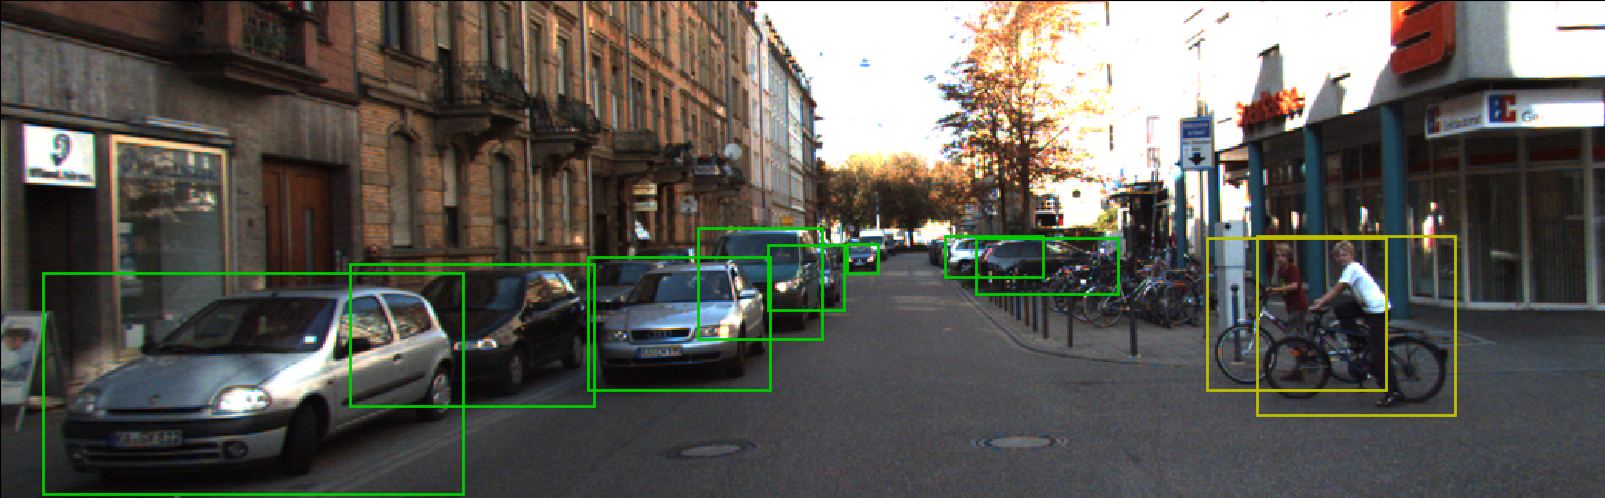
\includegraphics[width=0.8\textwidth]{images/detection_2d}\\
  				\caption{Example of 2D detection on KITTI dataset \cite{kitti}.}
  			\end{center}
  		\end{figure}
	  \end{itemize}
\end{frame}

\begin{frame}
	\frametitle{Motivation}
	\linespread{1.5}
	\begin{itemize}
		\item{In the context of autonomous driving, 2D bounding boxes are not sufficient:}
		\begin{itemize}
			\item{Lack of 3D pose and location.}
			\item{Occlusion.}
		\end{itemize}
		\item{The gap between 2D and 3D detections remains large due to:}
		\begin{itemize}
			\item{Adding a third dimension.}
			\item{Low resolution of 3D data.}
			\item {Deterioration of quality of 3D data as a function of distance.}
		\end{itemize}
	\end{itemize}
\end{frame}

\begin{frame}
	\frametitle{Motivation}
	\begin{figure}
		\begin{center}
			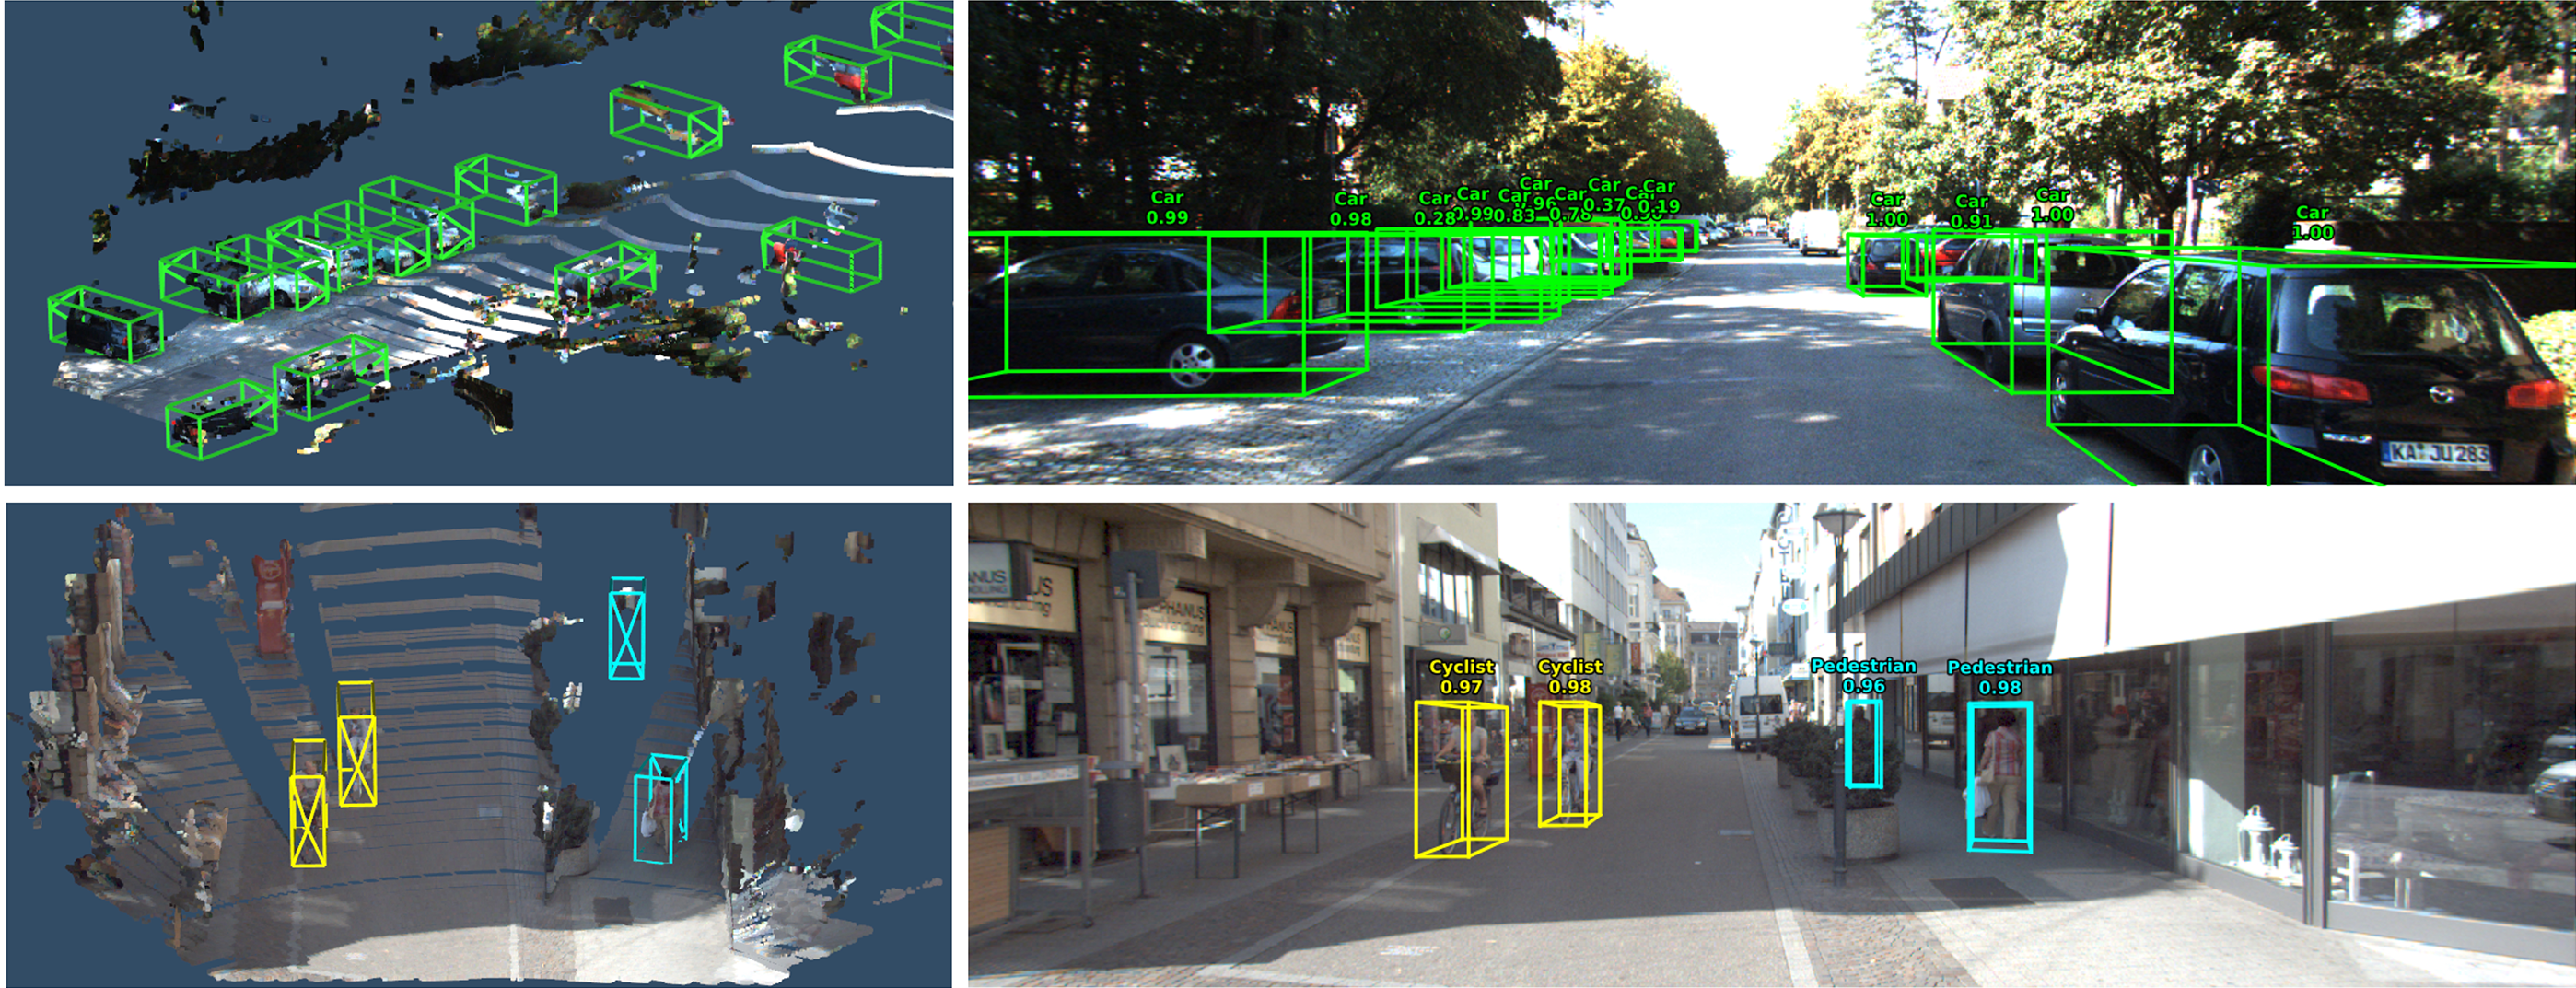
\includegraphics[width=1.0\textwidth]{images/Results_General}\\
			\caption{Example of 3D detection on KITTI dataset.}
		\end{center}
	\end{figure}
\end{frame}

\section{Problem Background}
\begin{frame}
	\frametitle{Background: Object Detection}
	\begin{figure}
		\begin{center}
			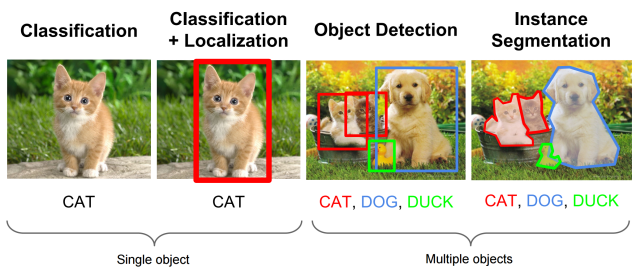
\includegraphics[width=1.0\textwidth]{images/LocalizationDetectionCuteness}\\
			\caption{Example of object classification, localization and segmentation \cite{object_det_cat}.}
		\end{center}
	\end{figure}
\end{frame}

\begin{frame}
	\frametitle{Background: Classic Object Detectors}
	\begin{itemize}
		\item{Most classical methods adopted the sliding-window technique which works by sliding a box around image and classifying each image
			crop inside a box.}
		\item{Pick a classifier (say SVM), run it at evenly spaced locations over the
			entire image, focusing on smaller areas of the feature map.}
	\end{itemize}
\end{frame}

\begin{frame}
	\frametitle{Background: Two-Stage Detection}
	\linespread{1.5}
	\begin{itemize}
		\item{The dominant paradigm in modern object.}
		\item{\textbf{First stage}: Generates
			a set of candidate proposals that should contain all the objects.}
		\item{\textbf{Second stage}: Classifies the object proposals and refines the location estimation of objects.}
	\end{itemize}
\end{frame}

\begin{frame}
	\frametitle{Background: Faster R-CNN}
	\begin{itemize}
		\item{Region Proposal Network (RPN)}
		\item{Region of interest pooling (RoI pooling)}
	\end{itemize}
	\begin{figure}
		\begin{center}
			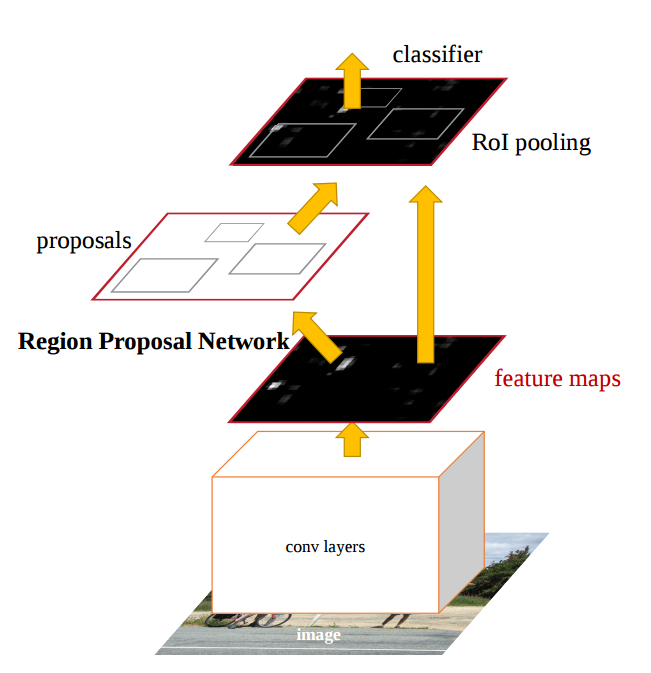
\includegraphics[width=0.5\textwidth]{images/faster_rcnn} \\
			\caption{Faster R-CNN architecture overview \cite{faster_rcnn}.}
		\end{center}
	\end{figure}
\end{frame}

% Too much text here
\begin{frame}
	\frametitle{Background: Single-Staged Detectors}
	\linespread{1.5}
	\begin{itemize}
		\item{Example architectures:}
		\begin{itemize}
			\item{OverFeat: Integrated Recognition, Localization and Detection using Convolutional Networks (Zhang et al - 2013)}
			\begin{itemize}
				\item{Multi-scale, sliding window approach}
			\end{itemize}
			\item{You Only Look Once: YOLO (Redmon et al - 2015)}
			\begin{itemize}
				\item{Discretizes the image into
					grids and then each grid cell proposes potential bounding boxes and scores those boxes
					using convolutional features.}
			\end{itemize}
			\item{Single Shot Detector: SSD (Liu et al - 2016)}
			\begin{itemize}
				\item{Discretizes the output space of bounding boxes into a set of default boxes over
					different aspect ratios and scales per feature map location}
			\end{itemize}
		\end{itemize}
	\end{itemize}
\end{frame}

\begin{frame}
	\frametitle{Background: Single-Stage Detection}
	\begin{itemize}
		\item{RPN free architectures.}
		\item{Example: You Only Look Once: YOLO (Redmon et al - 2015)}
		\begin{figure}
			\begin{center}
				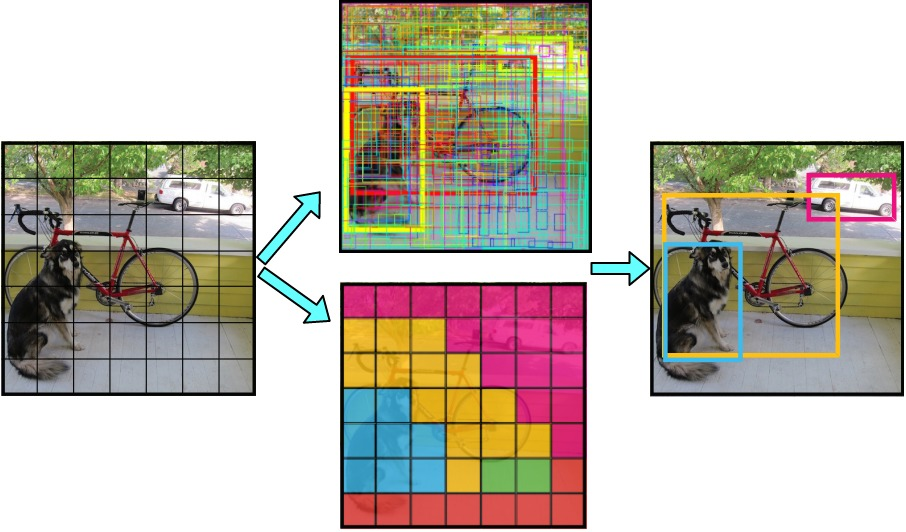
\includegraphics[width=0.8\linewidth]{images/yolo_concept} \\
				\caption{Yolo detection mechanism \cite{redmon2016you}.}
			\end{center}
		\end{figure}
	\end{itemize}
\end{frame}


\begin{frame}
	\frametitle{Background: 3D Object Detection}
	\linespread{1.5}
	\begin{itemize}
		\item{\textbf{3D RPN}: Generates a set of candidate 3D boxes.}
		\item{\textbf{Second stage}: Classifies and regresses the 3D boxes.}
		\item{Example architectures:}
		\begin{itemize}
			\item{\textbf{MV3D} - Multi-View 3D Object Detection Network for Autonomous Driving. (Chen et al 2017) \cite{mv3d}}
			\item{\textbf{F-PointNet} - Frustum PointNets for 3D Object Detection from RGB-D Data. (Qi et al 2018) \cite{frustumpointnet}}
		\end{itemize}
	\end{itemize}
\end{frame}

\begin{frame}
	\frametitle{Background: 3D Object Detector - MV3D \footnote{\tiny{ Multi-View 3D Object Detection Network for Autonomous Driving(CVPR) 2017.}}}
	\begin{center}
		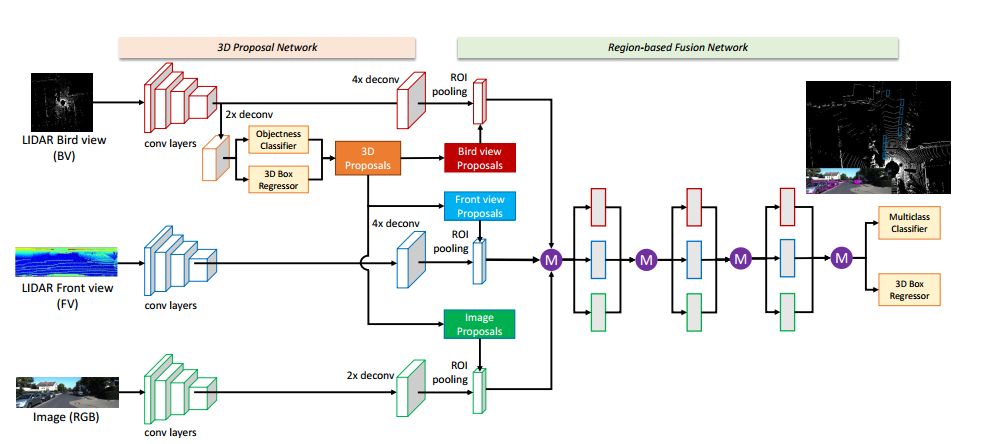
\includegraphics[width=1.0\textwidth]{images/mv3d_arch}
	\end{center}
	
\end{frame}

\begin{frame}
	\frametitle{Background: MV3D}
	\linespread{1.5}
	\begin{itemize}
		\item{A sensor fusion network.}
		\item{Encodes the sparse 3D point cloud into bird's eye view.}
		\item{\textbf{An RPN generates 3D candidate boxes from the bird's eye view representation.}}
		\item{\textbf{Uses 8 corner box representation to regress 3D bounding boxes.}}
	\end{itemize}
\end{frame}

\section{AVOD - Aggregate View Object Detection}
\begin{frame}
	\frametitle{AVOD - Aggregate View Object Detection}
	\begin{figure}
		\begin{center}
			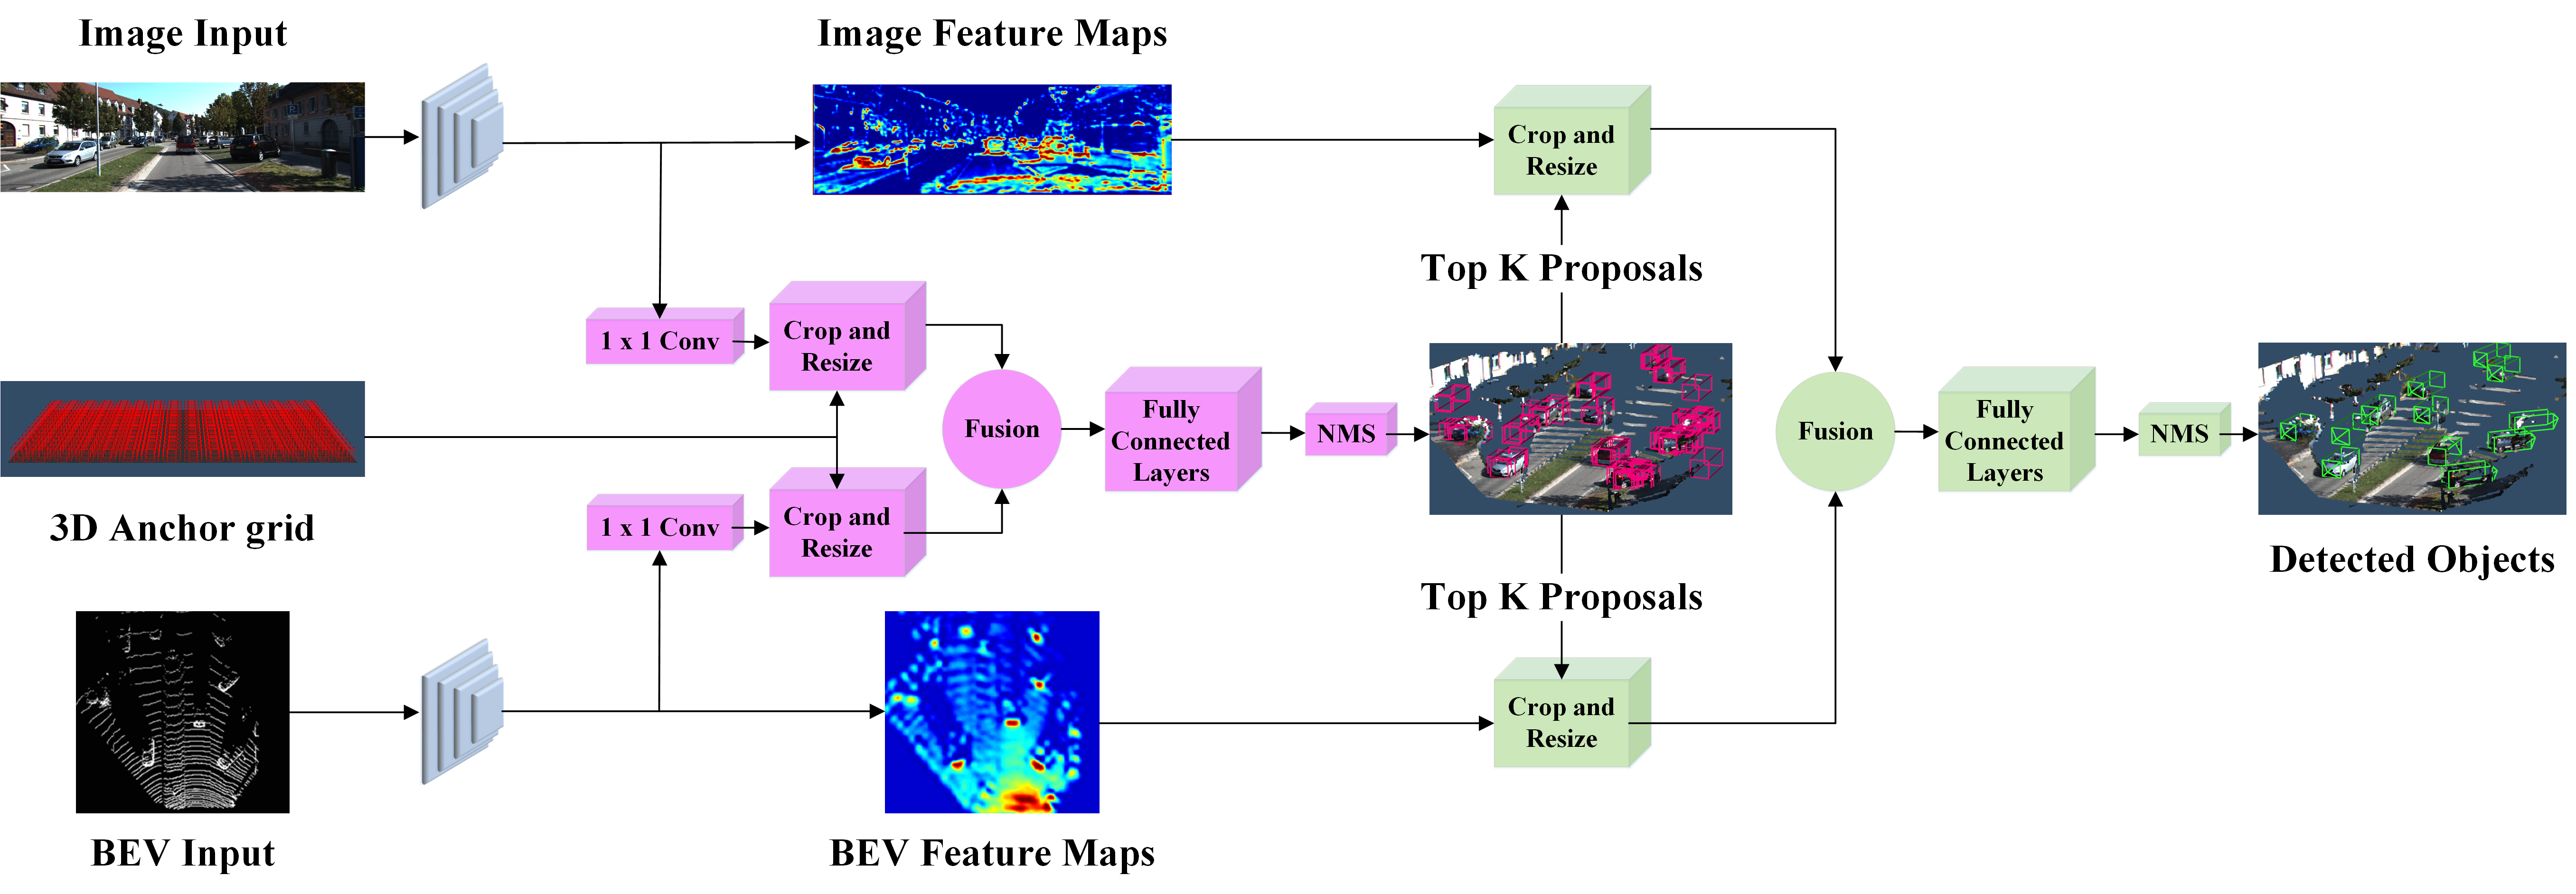
\includegraphics[width=115mm]{images/Meta-Architecture}
		\end{center}
	\caption{AVOD architectural diagram. The feature extractors are shown in \textbf{blue}, the region proposal network in \textbf{pink}, and the second stage detection network in \textbf{green}.}
	\end{figure}
\end{frame}

\begin{frame}
	\frametitle{AVOD - Aggregate View Object Detection}
	\begin{figure}
		\begin{center}
			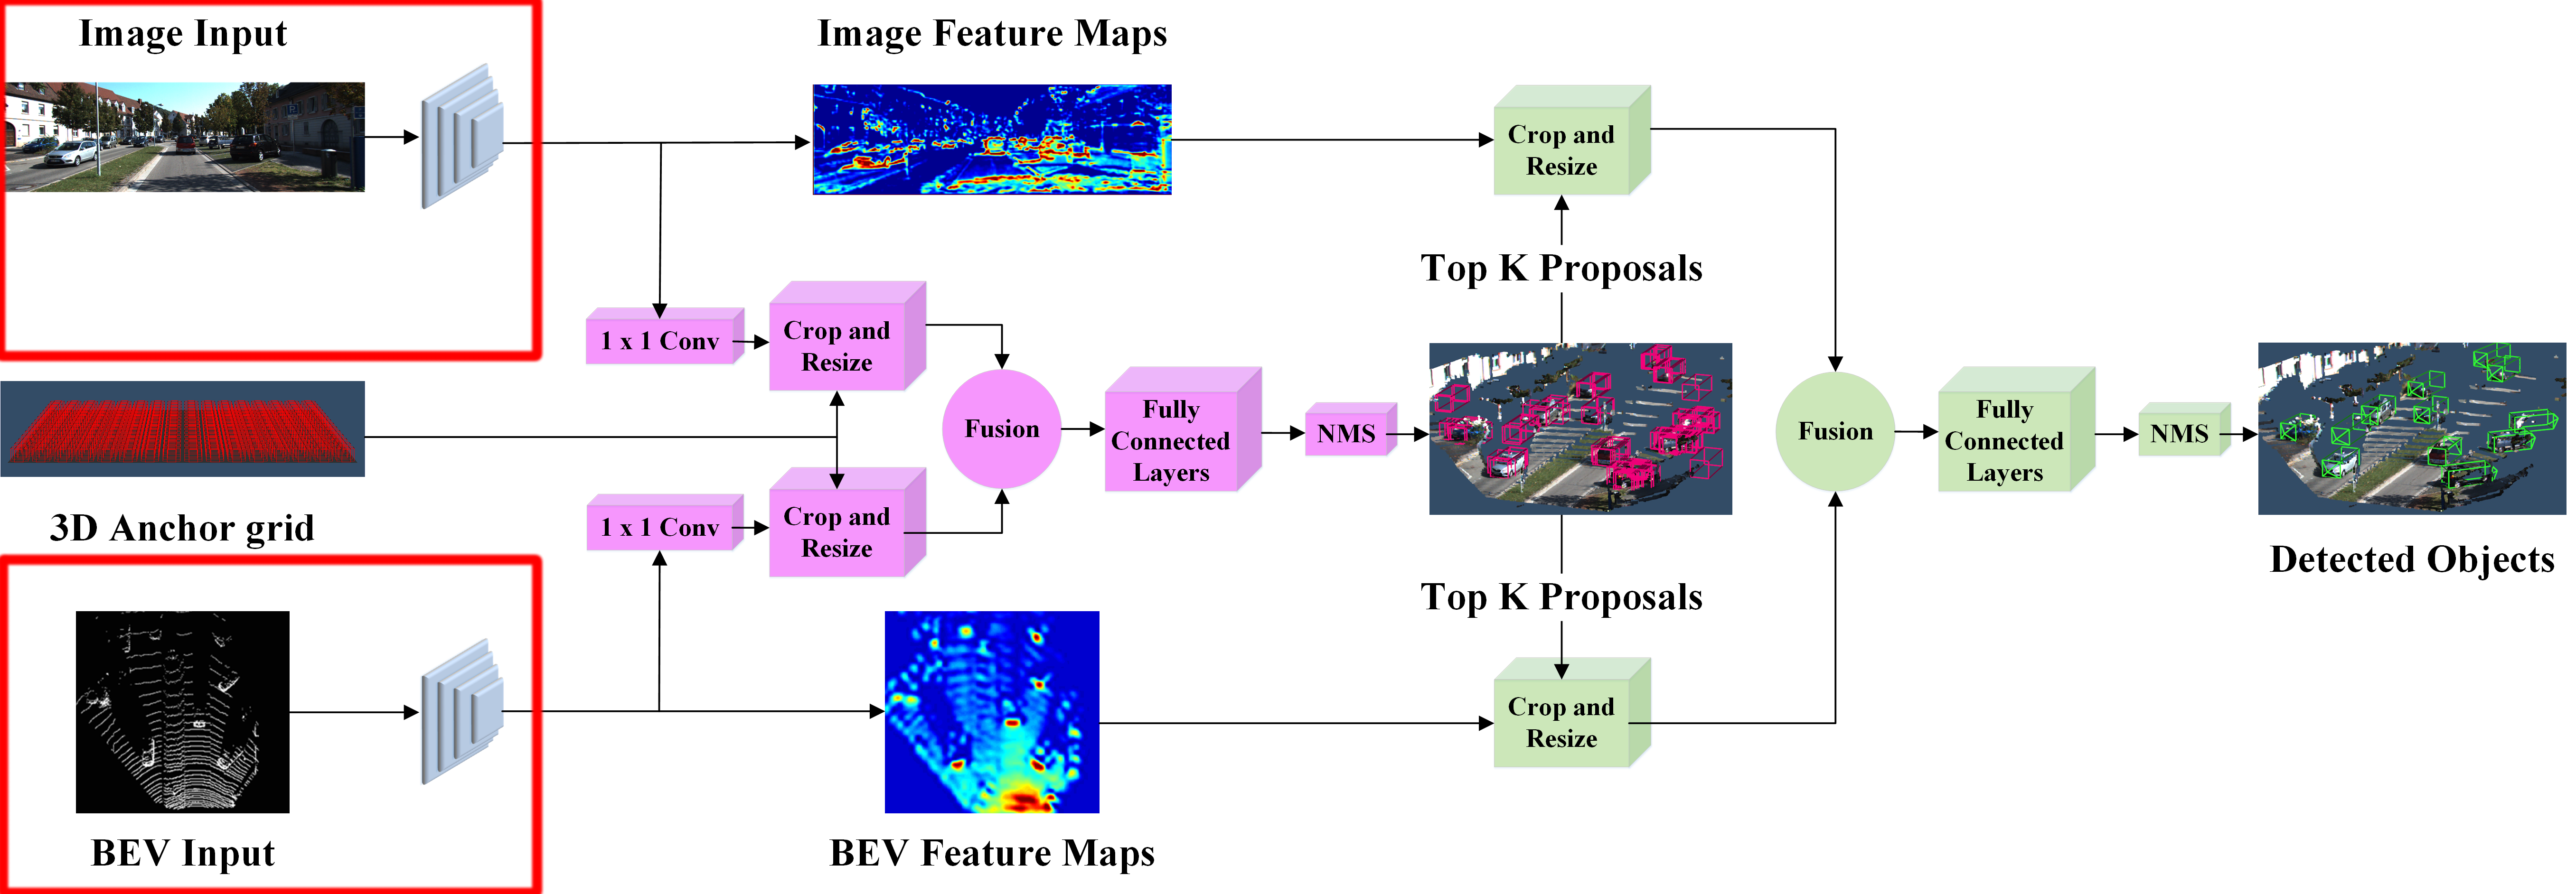
\includegraphics[width=115mm]{images/Meta-Architecture_1}
		\end{center}
		\caption{AVOD architectural diagram. The feature extractors are shown in \textbf{blue}, the region proposal network in \textbf{pink}, and the second stage detection network in \textbf{green}.}
	\end{figure}
\end{frame}


\begin{frame}
	\frametitle{AVOD - Input Data}
	\begin{itemize}
		\item{RGB Image}
		\\~\\
		\item{Bird's Eye View (\textbf{BEV}) Maps:}
		\\~\\
		\begin{itemize}
			\item{Small size variance.}
			\item{Small variance in vertical location.}
			\item{No issues with with occlusion.}
		\end{itemize}
	\end{itemize}
	\begin{picture}(200,130)
	\hspace{6.2cm}
		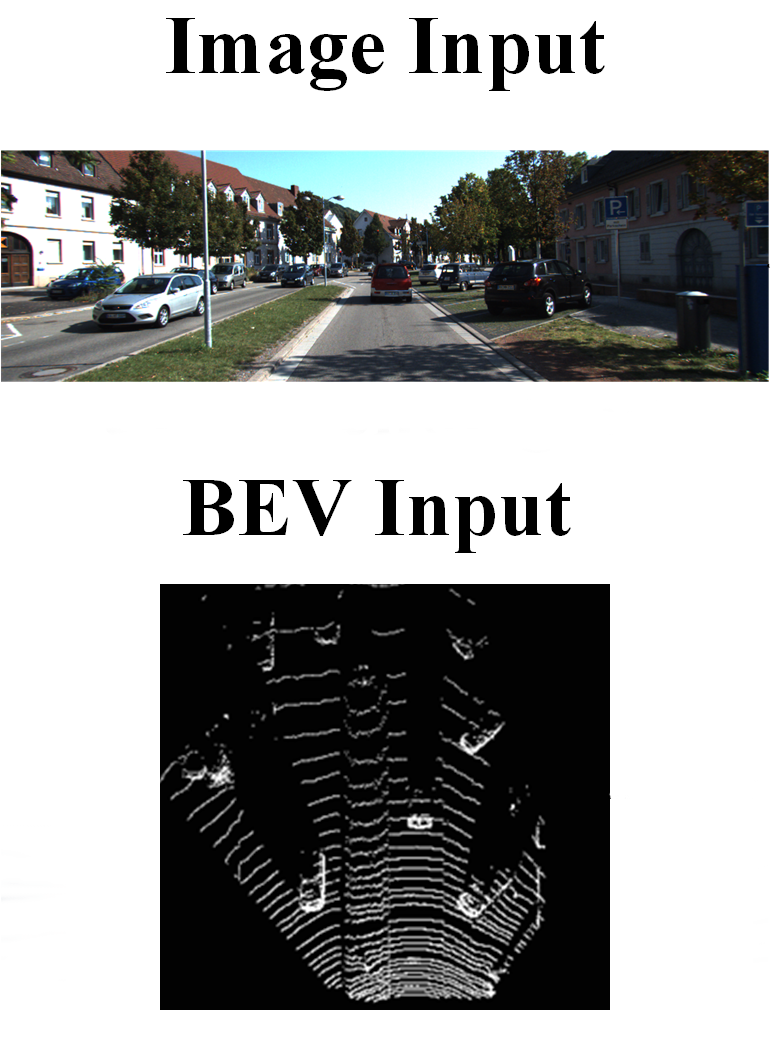
\includegraphics[width=0.5\linewidth]{images/Meta-Architecture_input}
	\end{picture}
\end{frame}

\begin{frame}
	\frametitle{Generating Feature Maps}
	\begin{itemize}
		\item{VGG Feature Extractor:}
	\end{itemize}
	\begin{figure}
		\begin{center}
			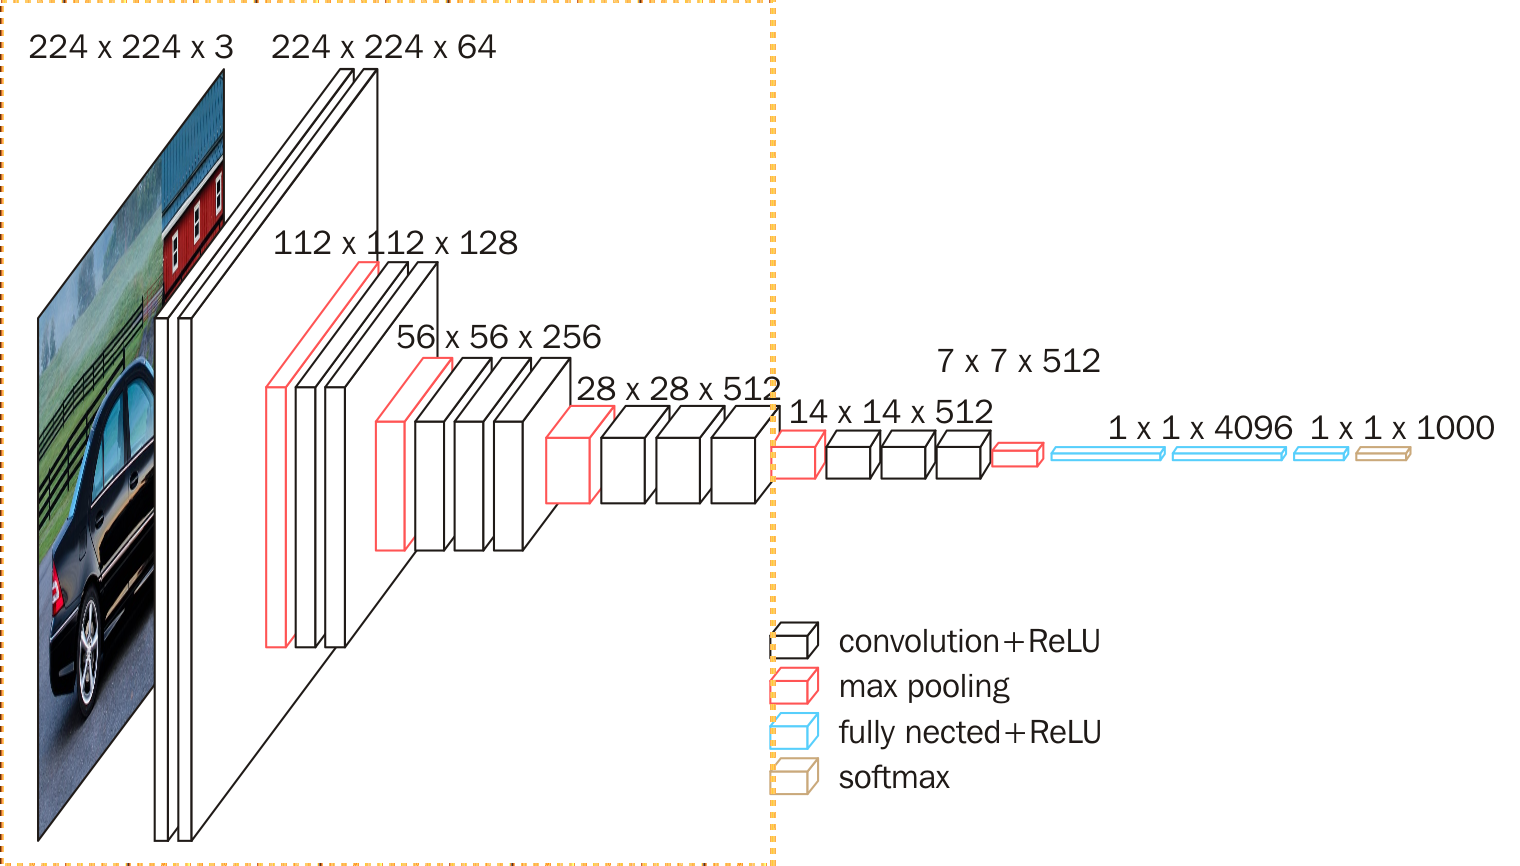
\includegraphics[width=0.7\linewidth]{images/vgg16} \\
			\caption{VGG16 architecture \cite{vgg_arch}.}
		\end{center}
	\end{figure}
	\begin{itemize}
		\item{Modified by resizing and reducing the layers.}
	\end{itemize}
\end{frame}

\begin{frame}
	\frametitle{Generating Feature Maps}
	\begin{itemize}
		\item{Feature Pyramid Feature Extractor}
	\end{itemize}
	\begin{figure}
	\begin{center}
		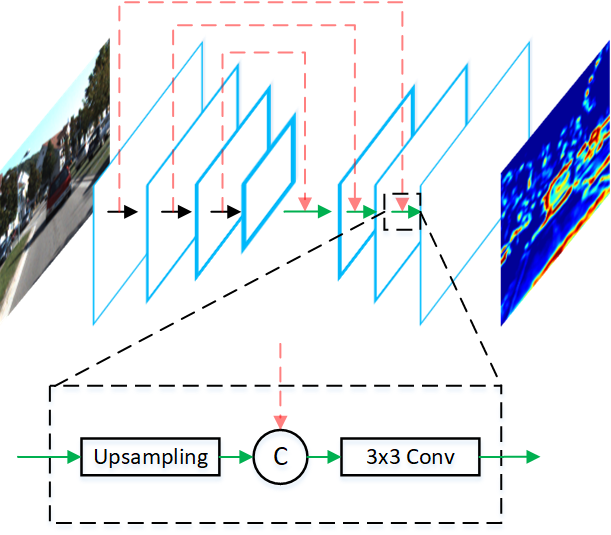
\includegraphics[width=0.5\linewidth]{images/Pyramid_Feature.png}
		\caption{Feature maps are fused at every layer by an \textit{upsampling} layer, followed by \textit{concatenation}, and then mixing via a \textit{convolutional} layer, resulting in a full resolution feature map.}
	\end{center}
	\end{figure}
\end{frame}


\begin{frame}
	\frametitle{RPN - Anchor Generation}
	\begin{figure}
		\begin{center}
			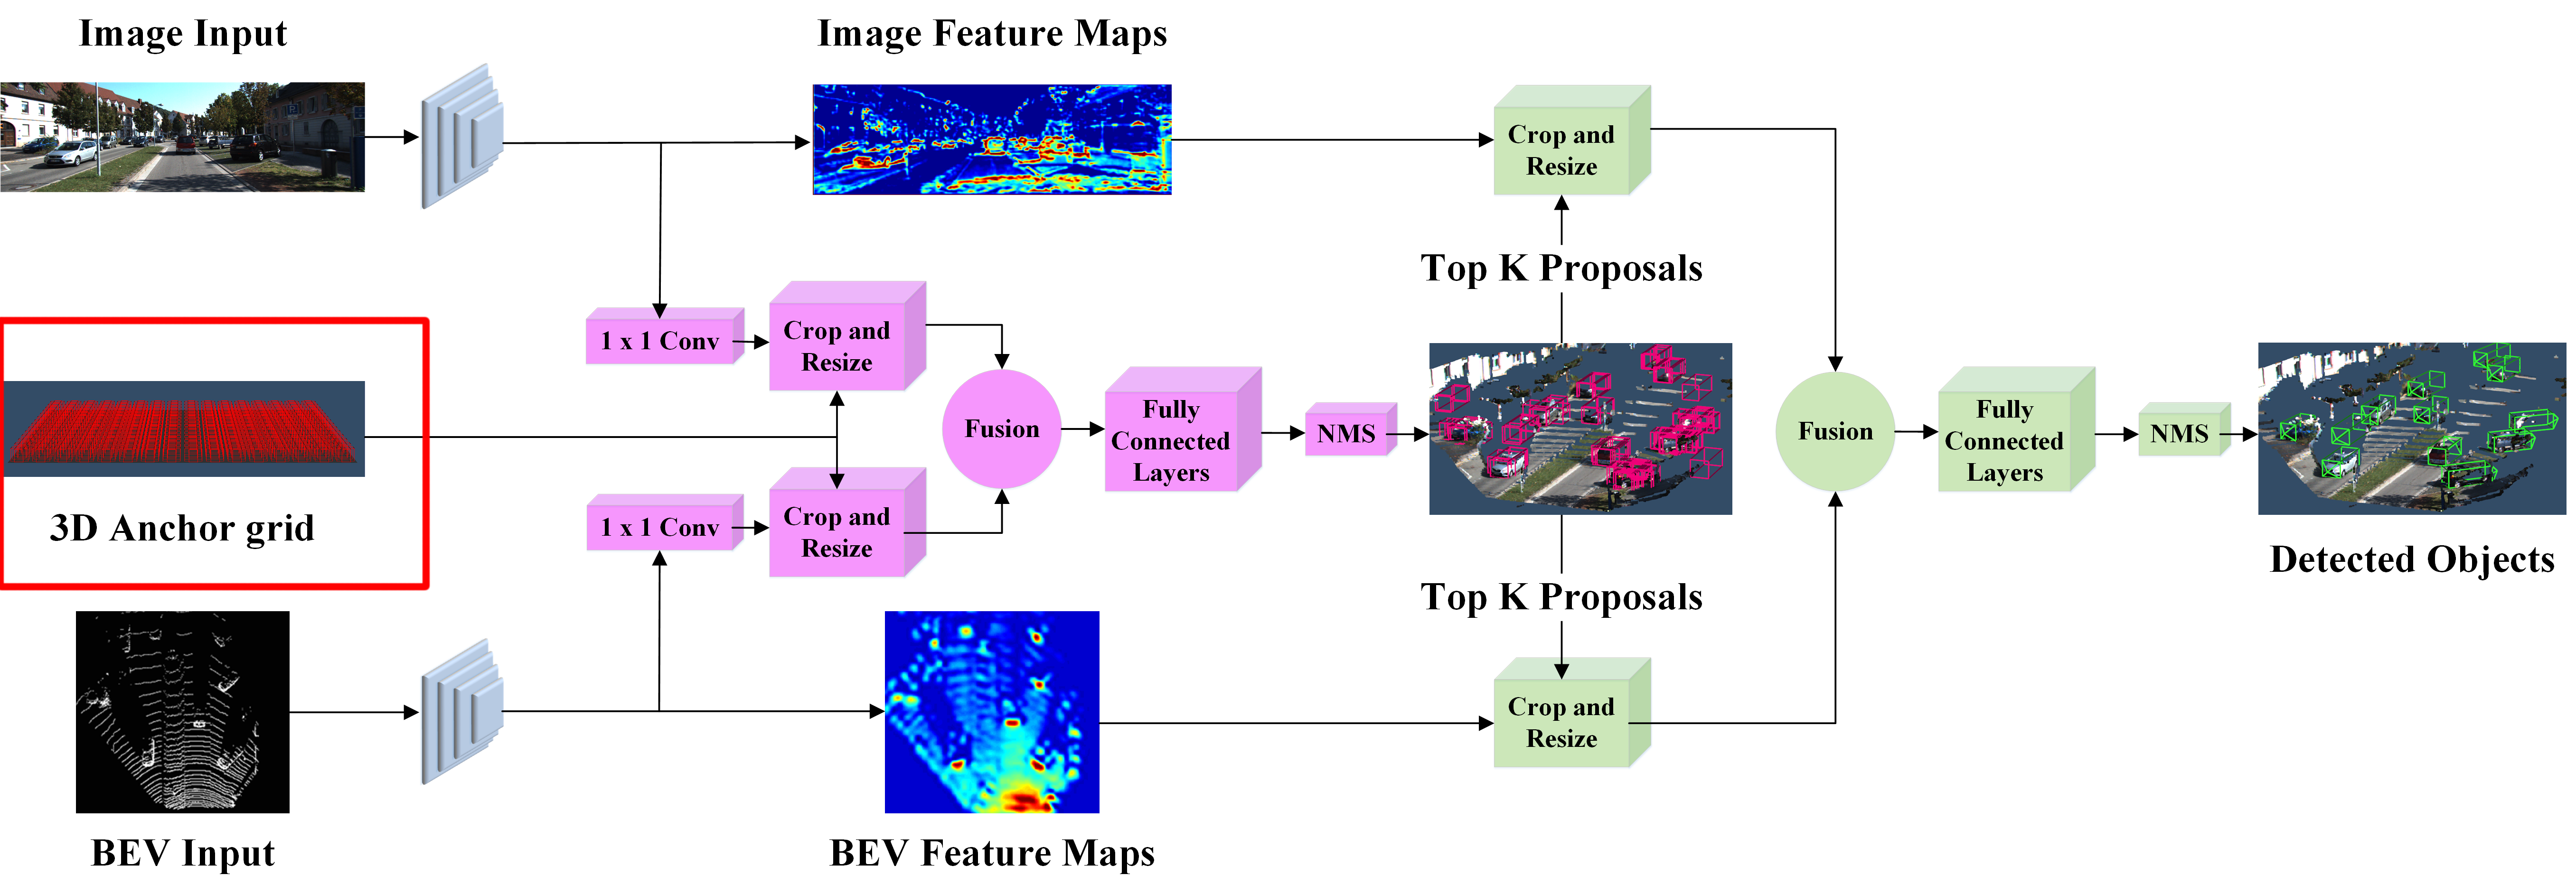
\includegraphics[width=115mm]{images/Meta-Architecture_2}
			\caption{AVOD architectural diagram. The feature extractors are shown in \textbf{blue}, the region proposal network in \textbf{pink}, and the second stage detection network in \textbf{green}.}
		\end{center}
	\end{figure}
\end{frame}	

\begin{frame}
	\frametitle{RPN - Anchor Generation}
	\begin{itemize}
		\item{\textbf{Anchors}: Initial guesses on where objects are located.}
		\begin{itemize}
			\item{Encoded as $[x, y, z, l, w, h]$}
		\end{itemize}
		\item{Take 3D box sizes from ground truth clusters.}
		\item{Generated on a grid on the ground plane, with $0^\circ$ or $90^\circ$ orientations.}
	\end{itemize}
	\begin{figure}[H]
		\begin{center}
			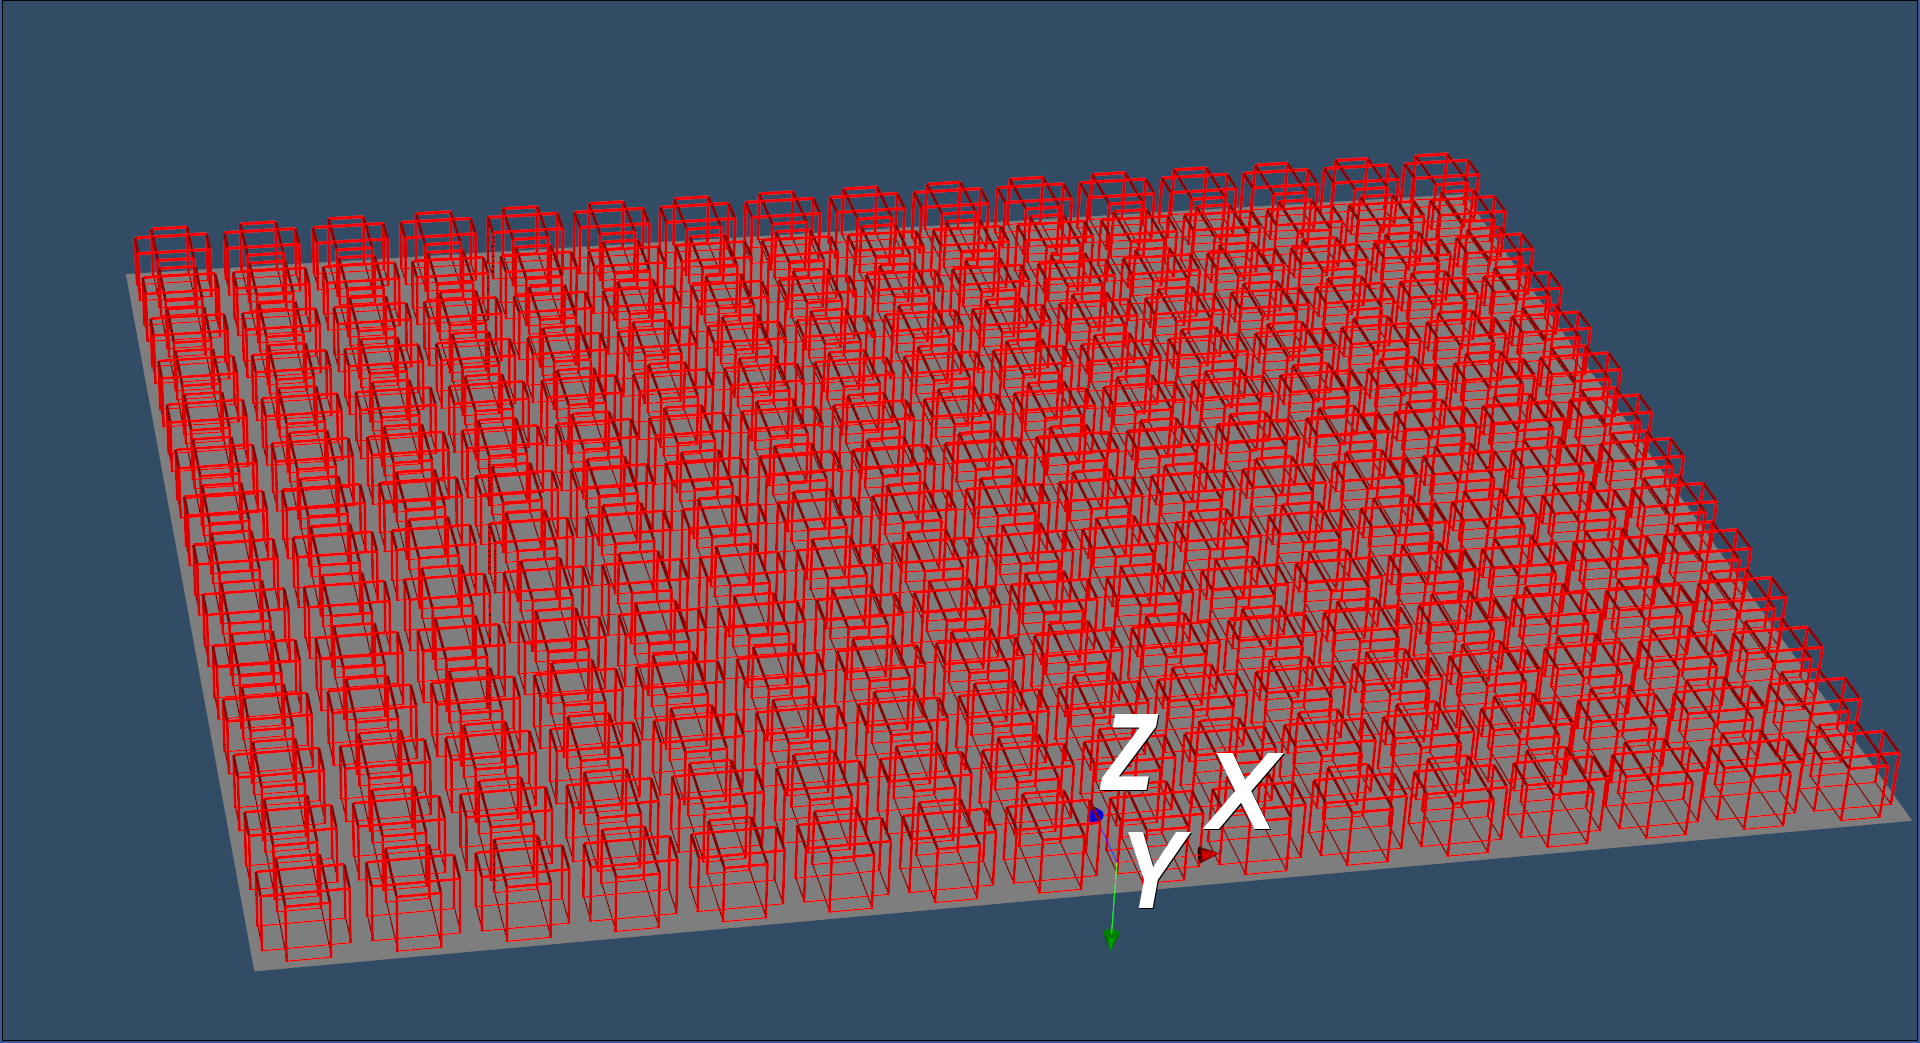
\includegraphics[width=0.6\linewidth]{images/anchor_grid}
			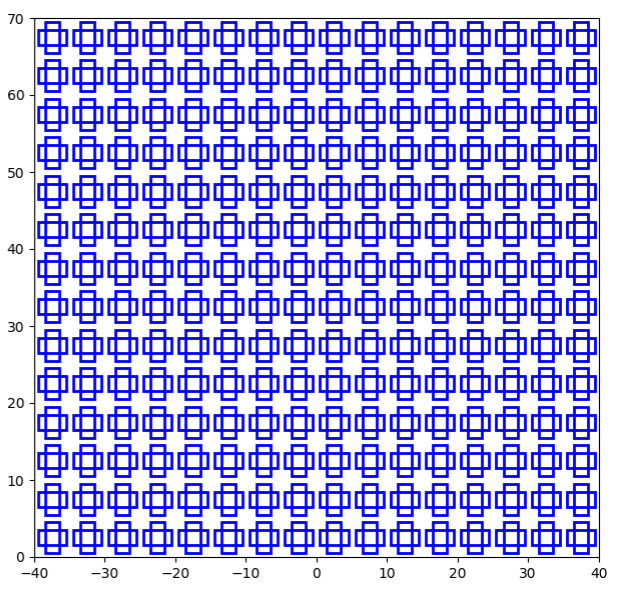
\includegraphics[width=0.4\linewidth]{images/projected_anchors_in_bev}
		\end{center}
		\caption{Left: Example of anchor grid with 1 cluster, and $5m$ stride. Right: Example of anchors projected into Bird's Eye View.}
	\end{figure}
\end{frame}

\begin{frame}
	\frametitle{Region Proposal Network}
	\begin{figure}
		\begin{center}
			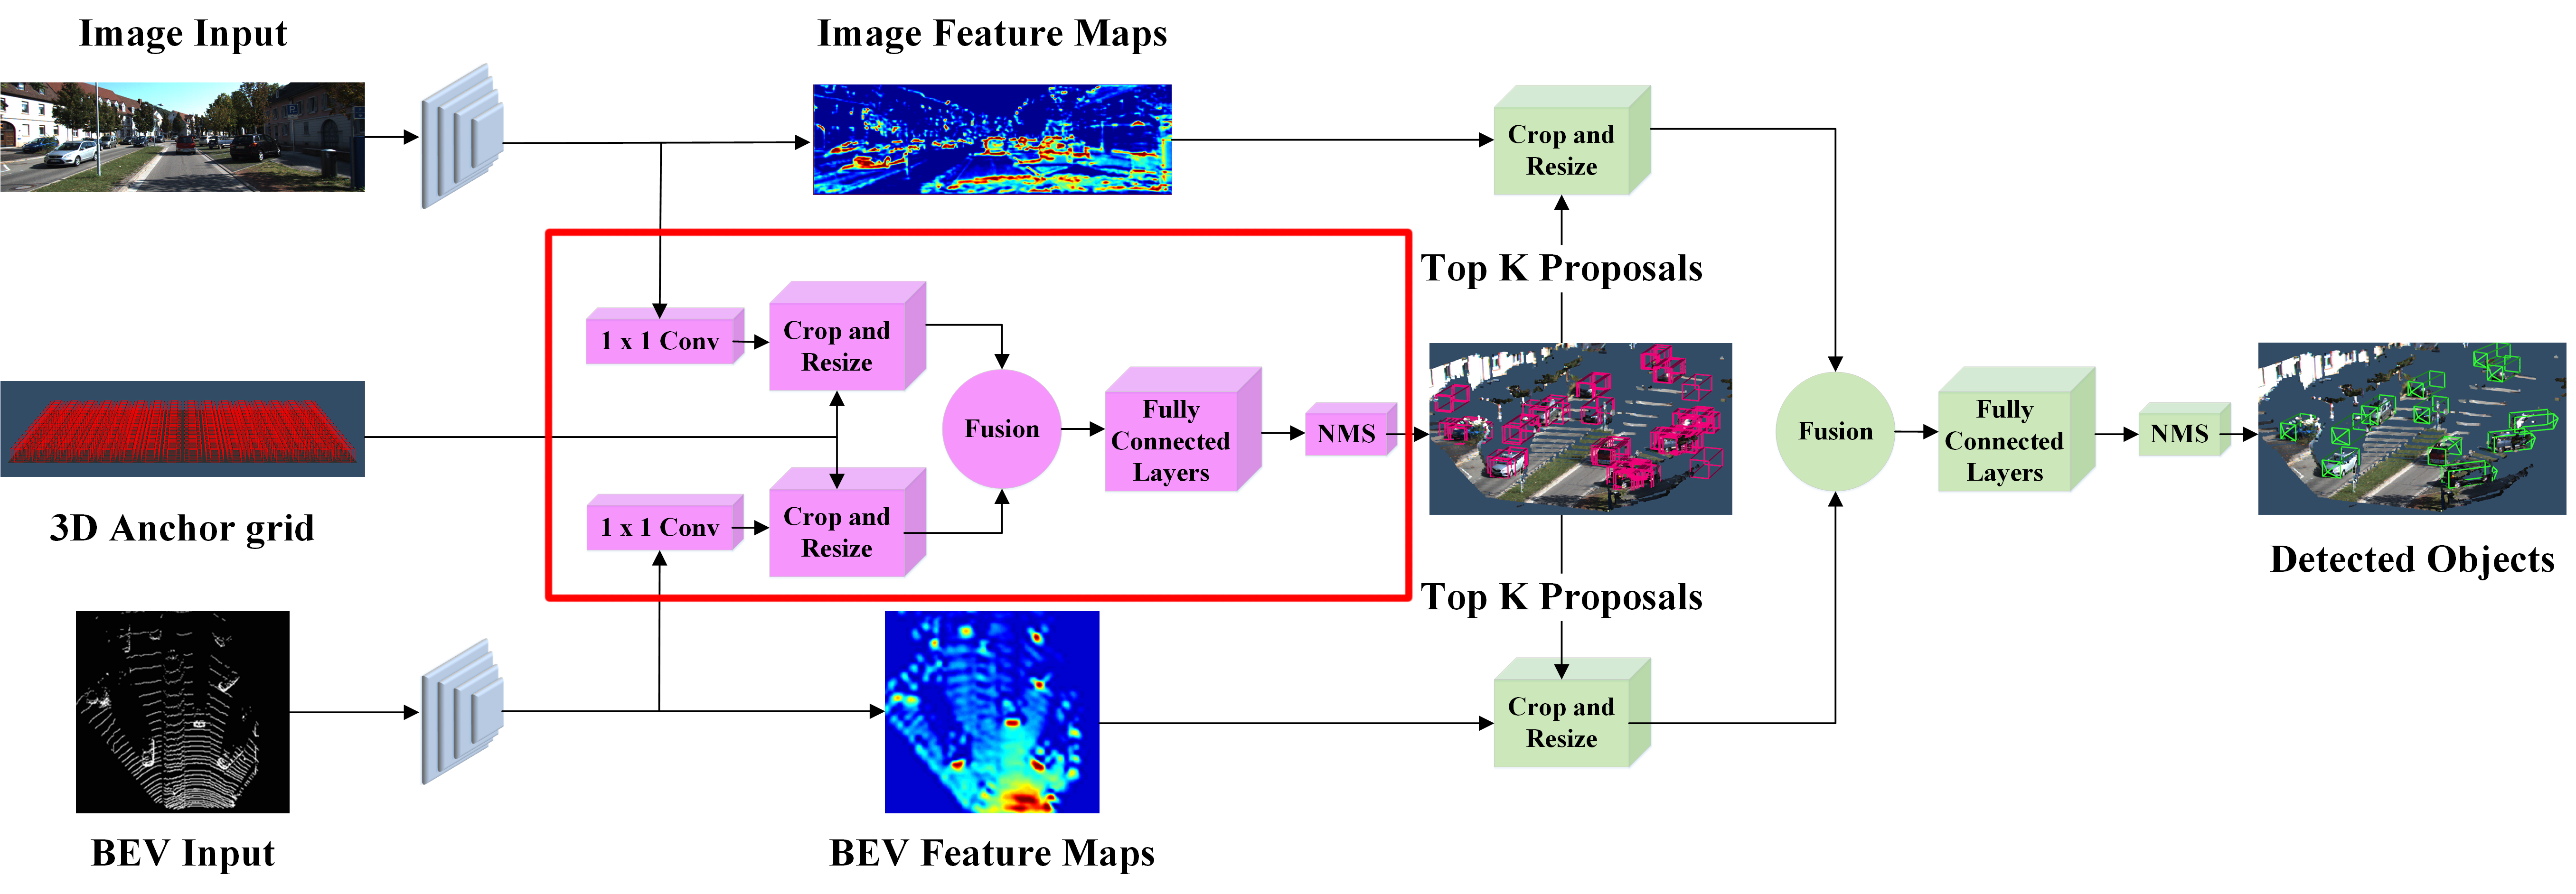
\includegraphics[width=115mm]{images/Meta-Architecture_3}
			\caption{AVOD architectural diagram. The feature extractors are shown in \textbf{blue}, the region proposal network in \textbf{pink}, and the second stage detection network in \textbf{green}.}
		\end{center}
	\end{figure}
\end{frame}	

\begin{frame}
	\frametitle{Region Proposal Network}
	\begin{figure}[H]
		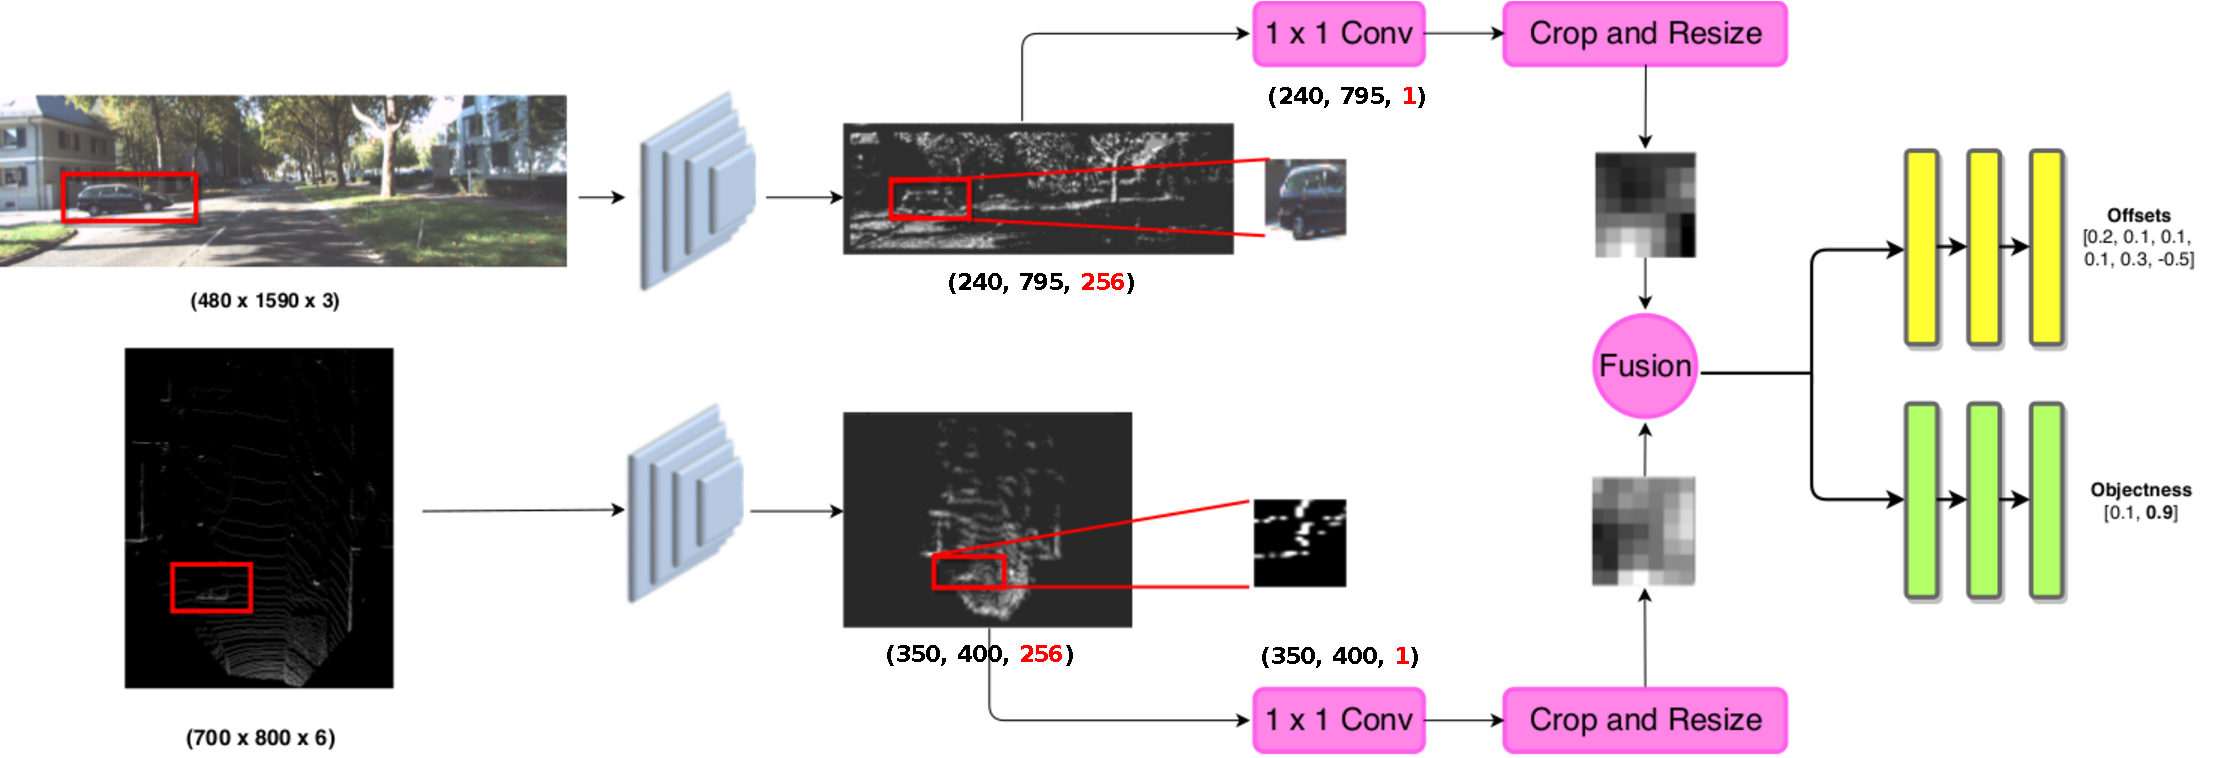
\includegraphics[width=115mm]{images/pdfs/rpn_crop_resize}
		\caption{RPN fusion \& proposal generation.}
	\end{figure}
\end{frame}


\begin{frame}
	\frametitle{Second Stage Detection Network}
	\begin{figure}
		\begin{center}
			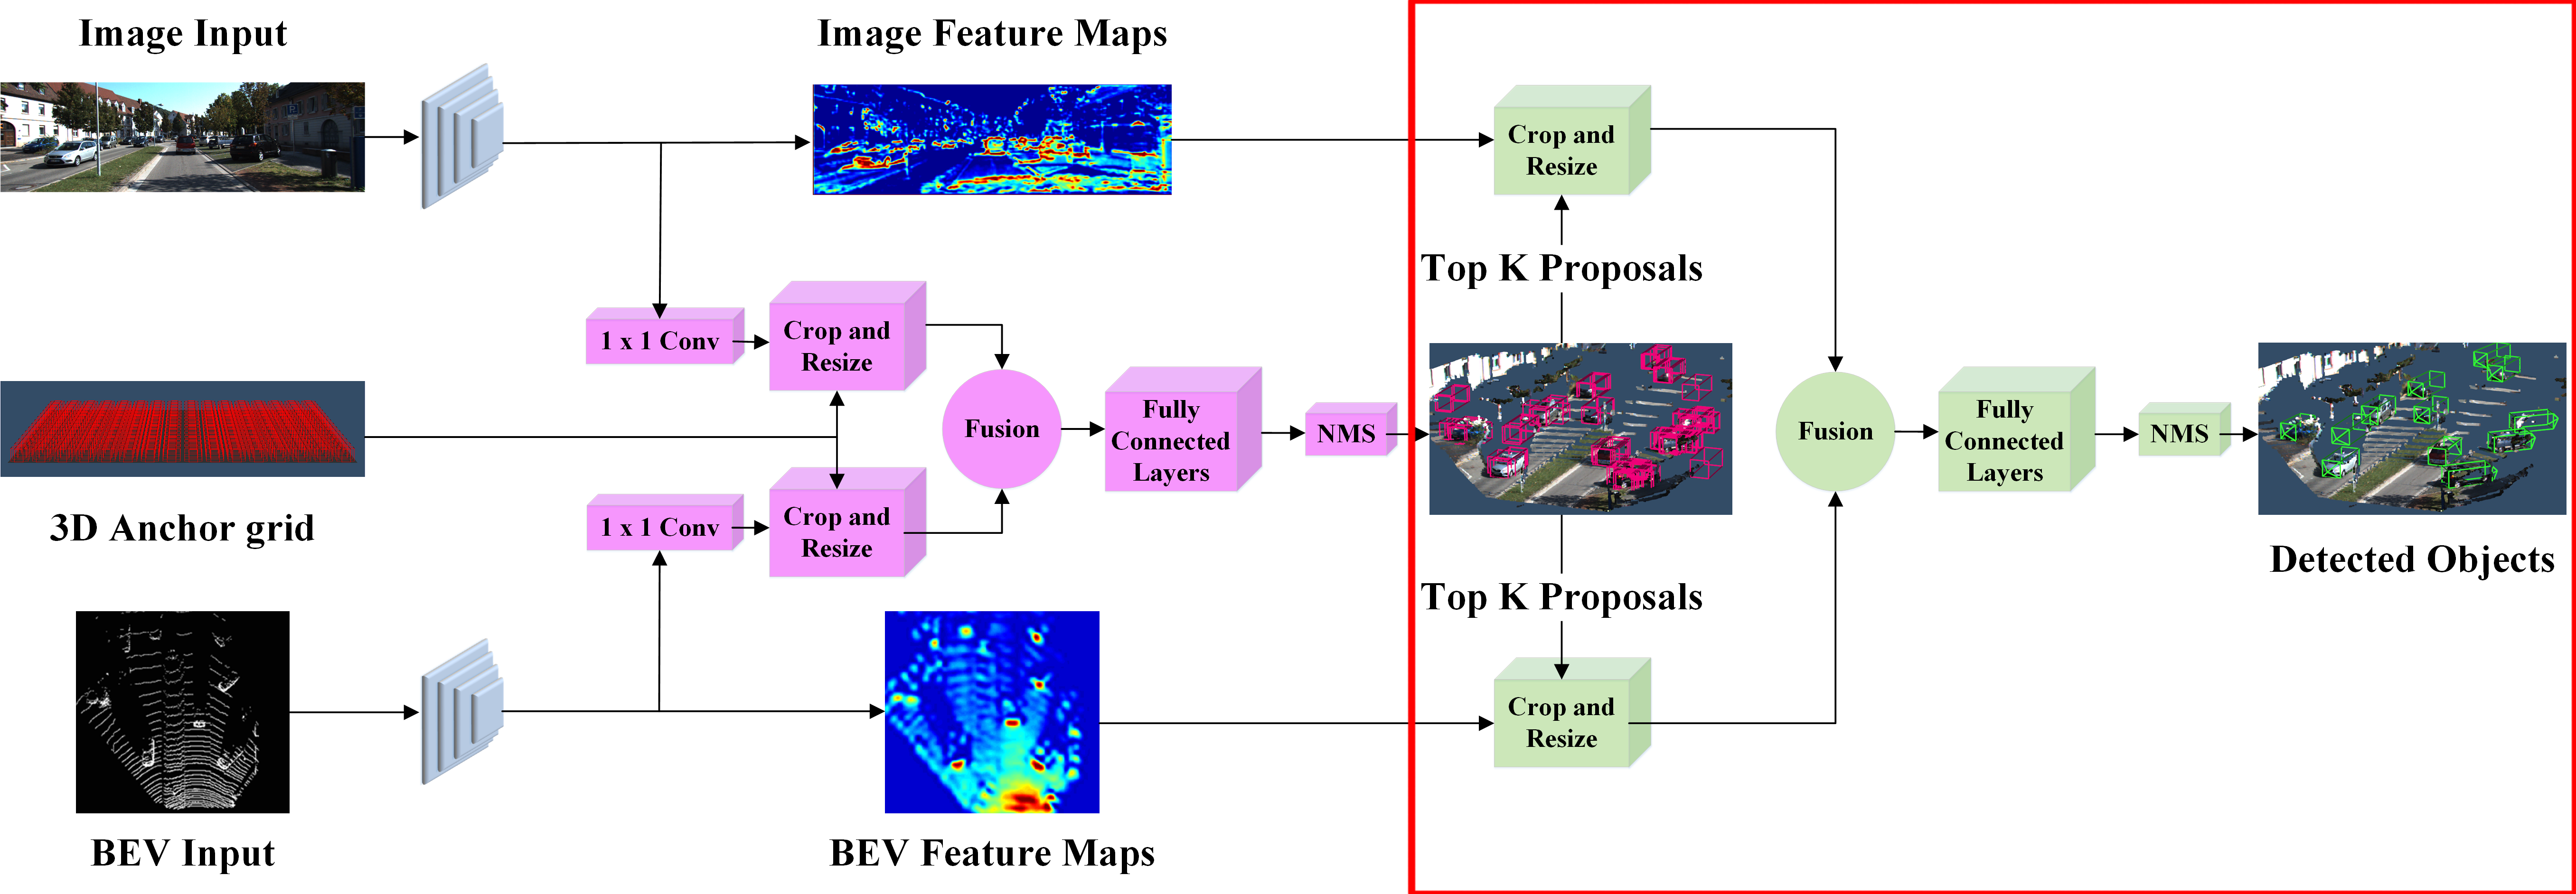
\includegraphics[width=115mm]{images/Meta-Architecture_4}
			\caption{AVOD architectural diagram. The feature extractors are shown in \textbf{blue}, the region proposal network in \textbf{pink}, and the second stage detection network in \textbf{green}.}
		\end{center}
	\end{figure}
\end{frame}	

\begin{frame}
	\frametitle{Second Stage Detection Network}
	\begin{itemize}
		\item{3D Bounding Box Encoding}
		\begin{itemize}
			\item{\textbf{Four corners and two heights}.}
		\end{itemize}
	\end{itemize}
	\begin{figure}[h] 
		\begin{center}
			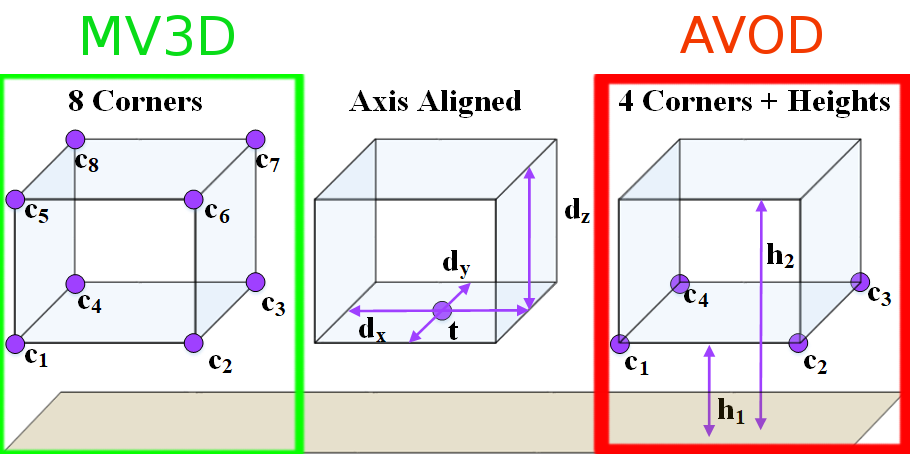
\includegraphics[width=0.7\textwidth]{images/box_encodings.png}
		\end{center}
		\caption{A visual comparison between the $8$ corner box encoding, the axis aligned box encoding and AVOD's $4$ corner encoding.}
		\label{encoding}
	\end{figure}
\end{frame}

\begin{frame}
	\frametitle{Explicit Orientation Vector Regression}
	\begin{itemize}
		\item{AVOD remedies this by computing: $(x_{or}, y_{or})= (\cos(\theta),\sin(\theta))$}
		\item{Handles angle wrapping as every $\theta \in [-\pi, \pi]$ can be represented
			by a unique unit vector in the BEV space.}
	\end{itemize}
	\begin{figure}
		\begin{center}
			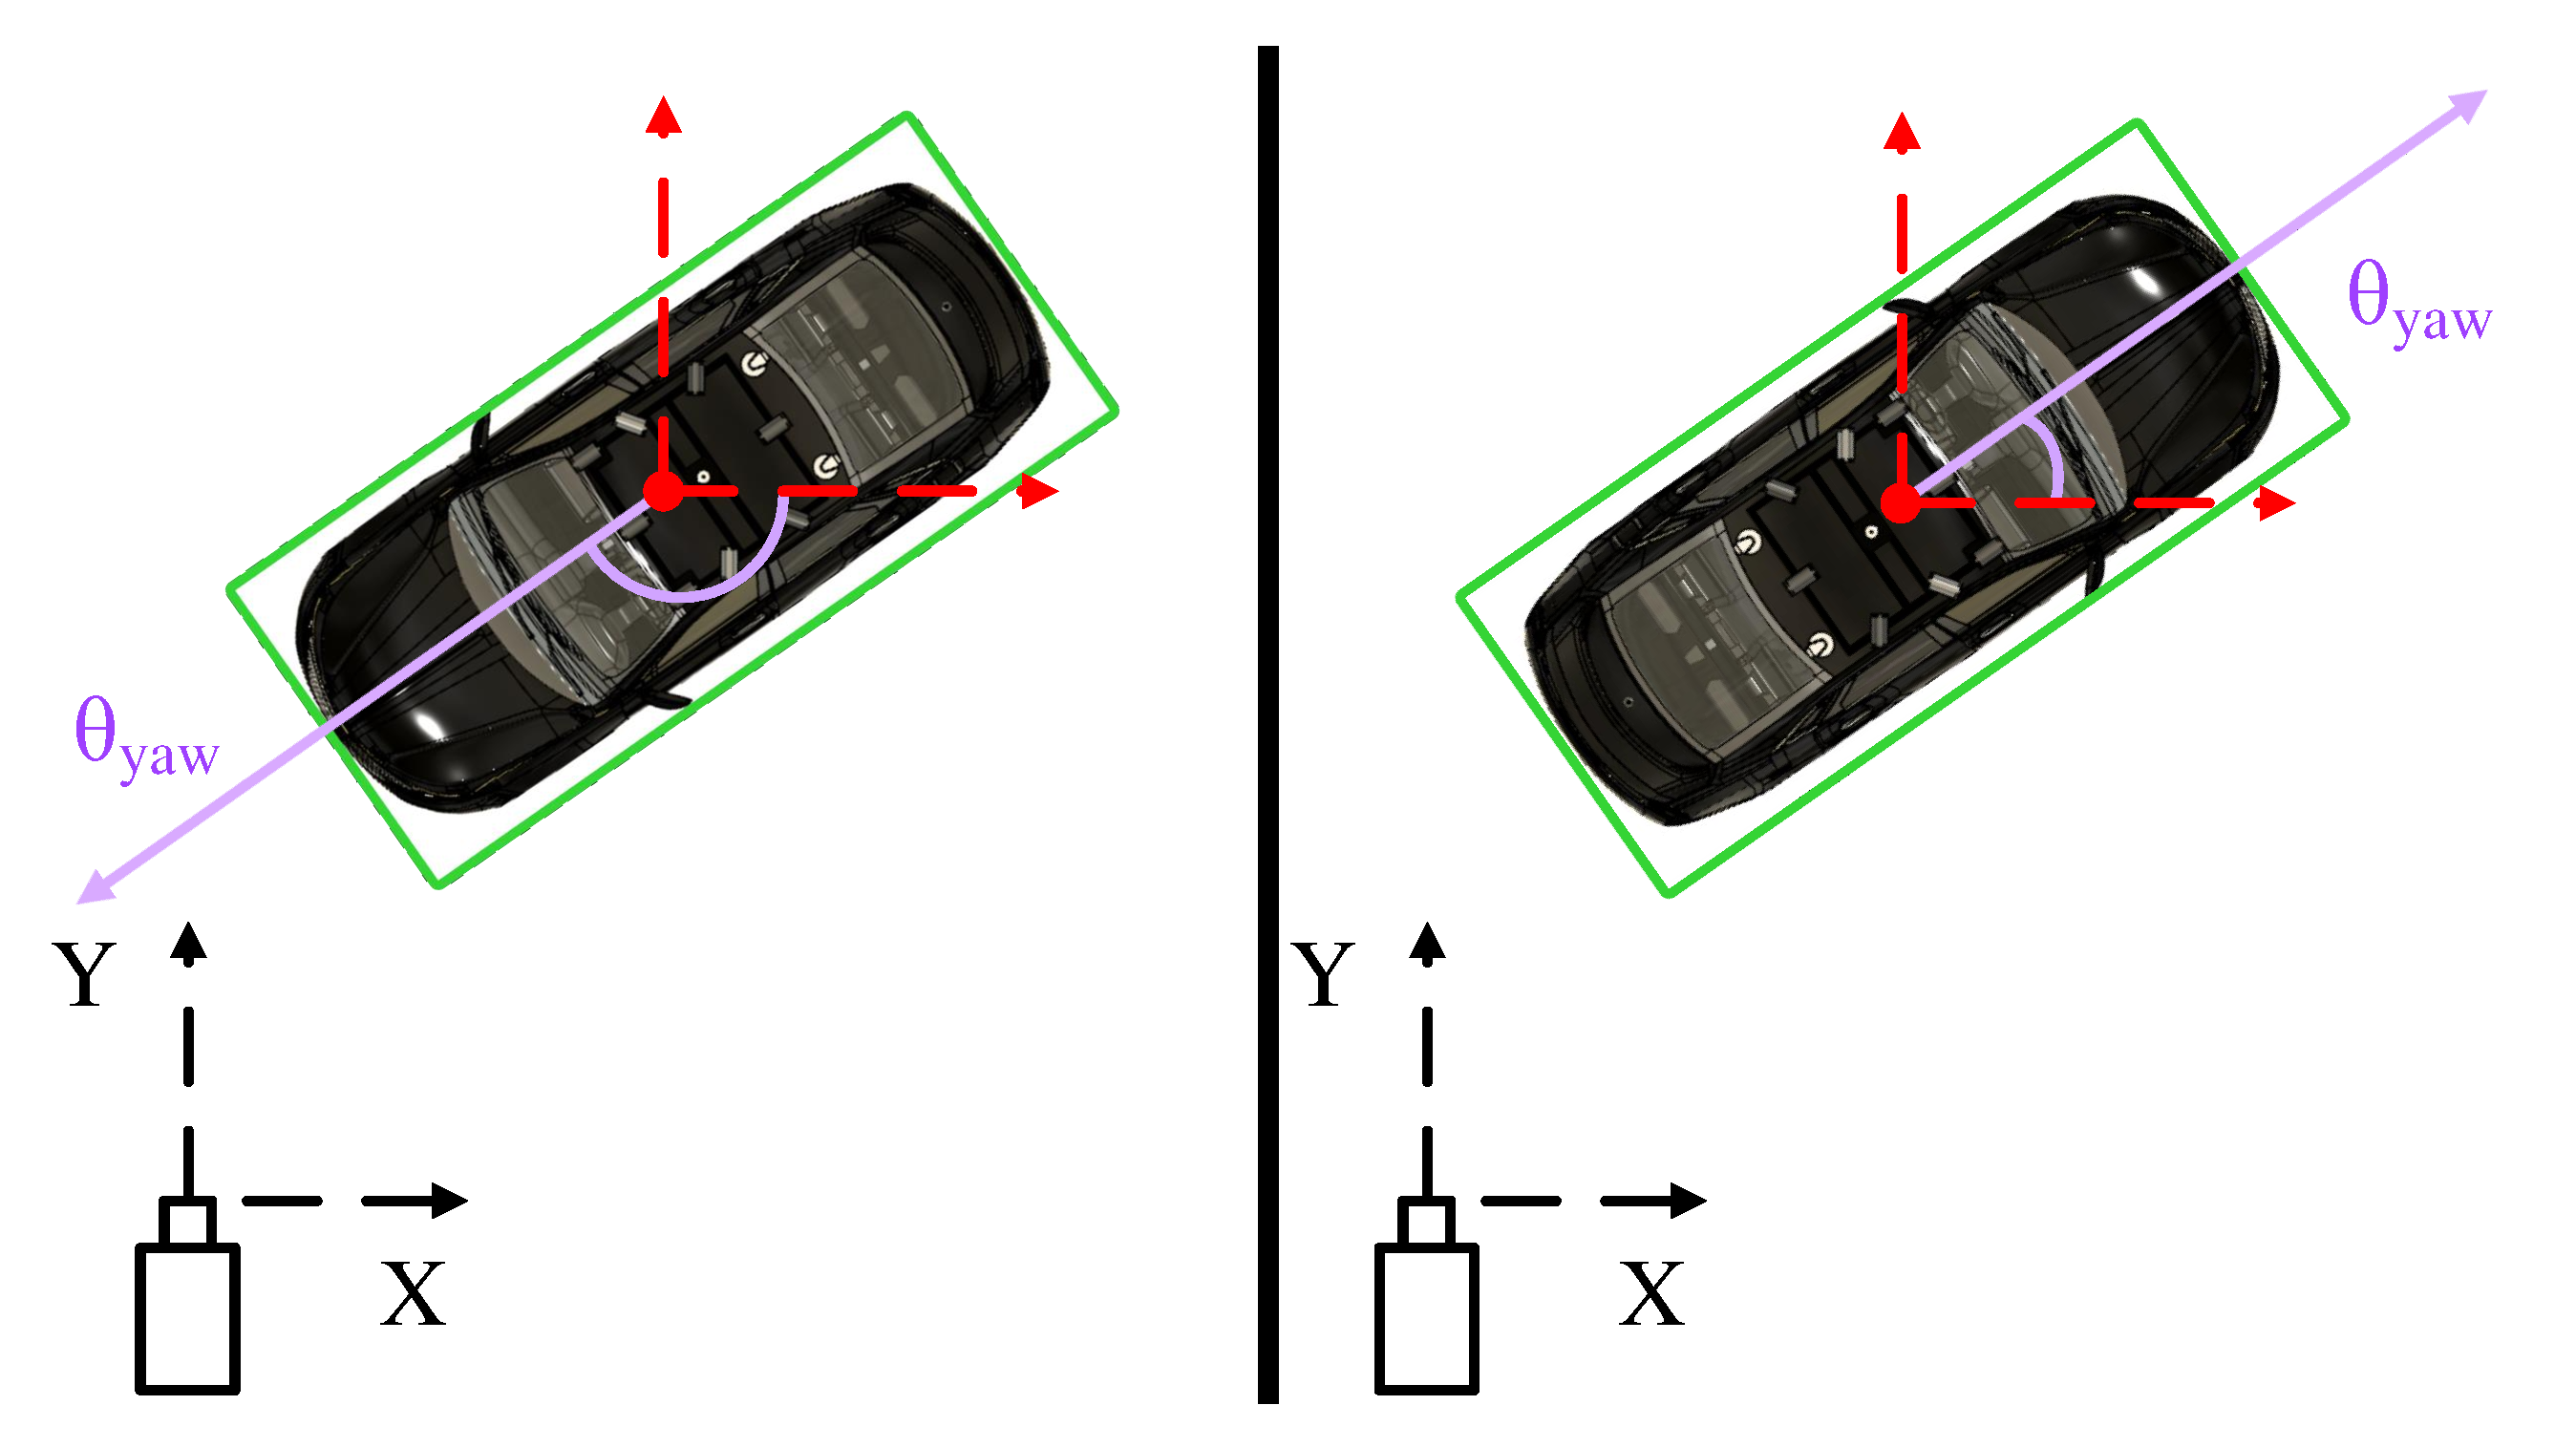
\includegraphics[width=0.7\textwidth]{images/pdfs/Metric.pdf}	
			\caption{Object's bounding box does not change when the orientation (\textbf{purple}) is shifted by $\pm \pi$ radians.}
		\end{center}
	\end{figure}
\end{frame}

\begin{frame}
	\frametitle{Second Stage Detection Network}
	\begin{figure}
		\begin{center}
			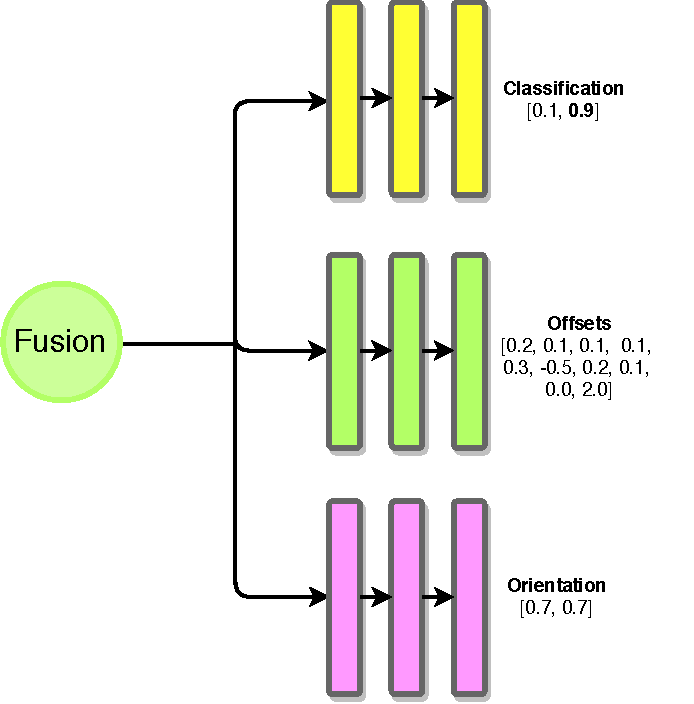
\includegraphics[width=0.5\textwidth]{images/pdfs/second_fusion}
			\caption{AVOD second stage task specific layers.}
		\end{center}
	\end{figure}
\end{frame}	

\begin{frame}
	\frametitle{Orientation Ambiguity}
	\begin{figure}
		\begin{center}
			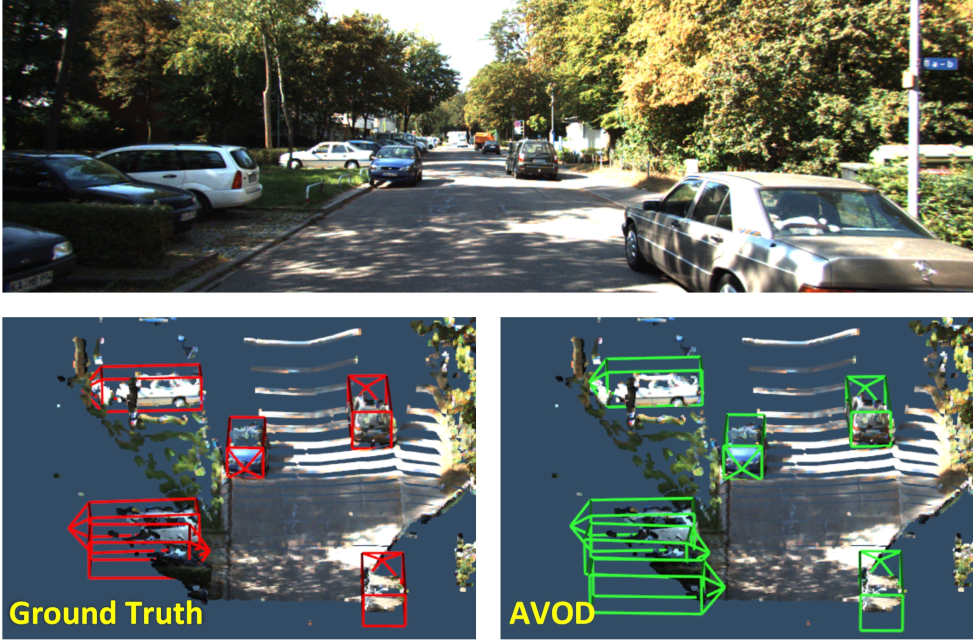
\includegraphics[width=0.6\textwidth]{images/avod_detec_gt}\\
			\hspace{-1cm}
			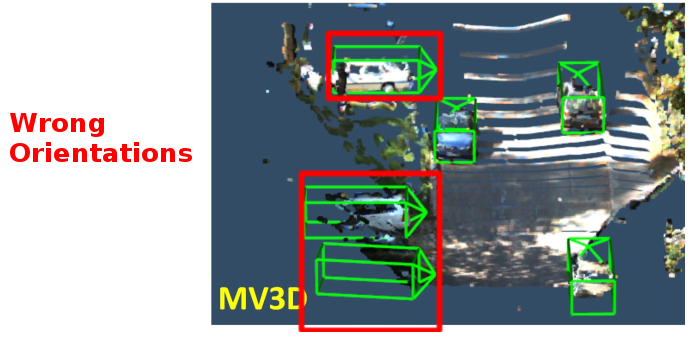
\includegraphics[width=0.44\textwidth]{images/mv3dwrong}
			\caption{Qualitative comparison between MV3D and AVOD.}	
		\end{center}
	\end{figure}
\end{frame}

\begin{frame}
	\frametitle{Evaluation Metrics for Object Detection}
	\begin{itemize}
		\item{Precision \& Recall}
	\begin{center}
		\begin{align*}
		Precision = \frac{TP}{TP + FP} \quad \quad Recall = \frac{TP}{TP + FN}
		\end{align*}
	\end{center}
	\end{itemize}
\end{frame}

\begin{frame}
	\frametitle{RPN Input Variations}
	\begin{figure}
		\hspace{-1.16cm} 
			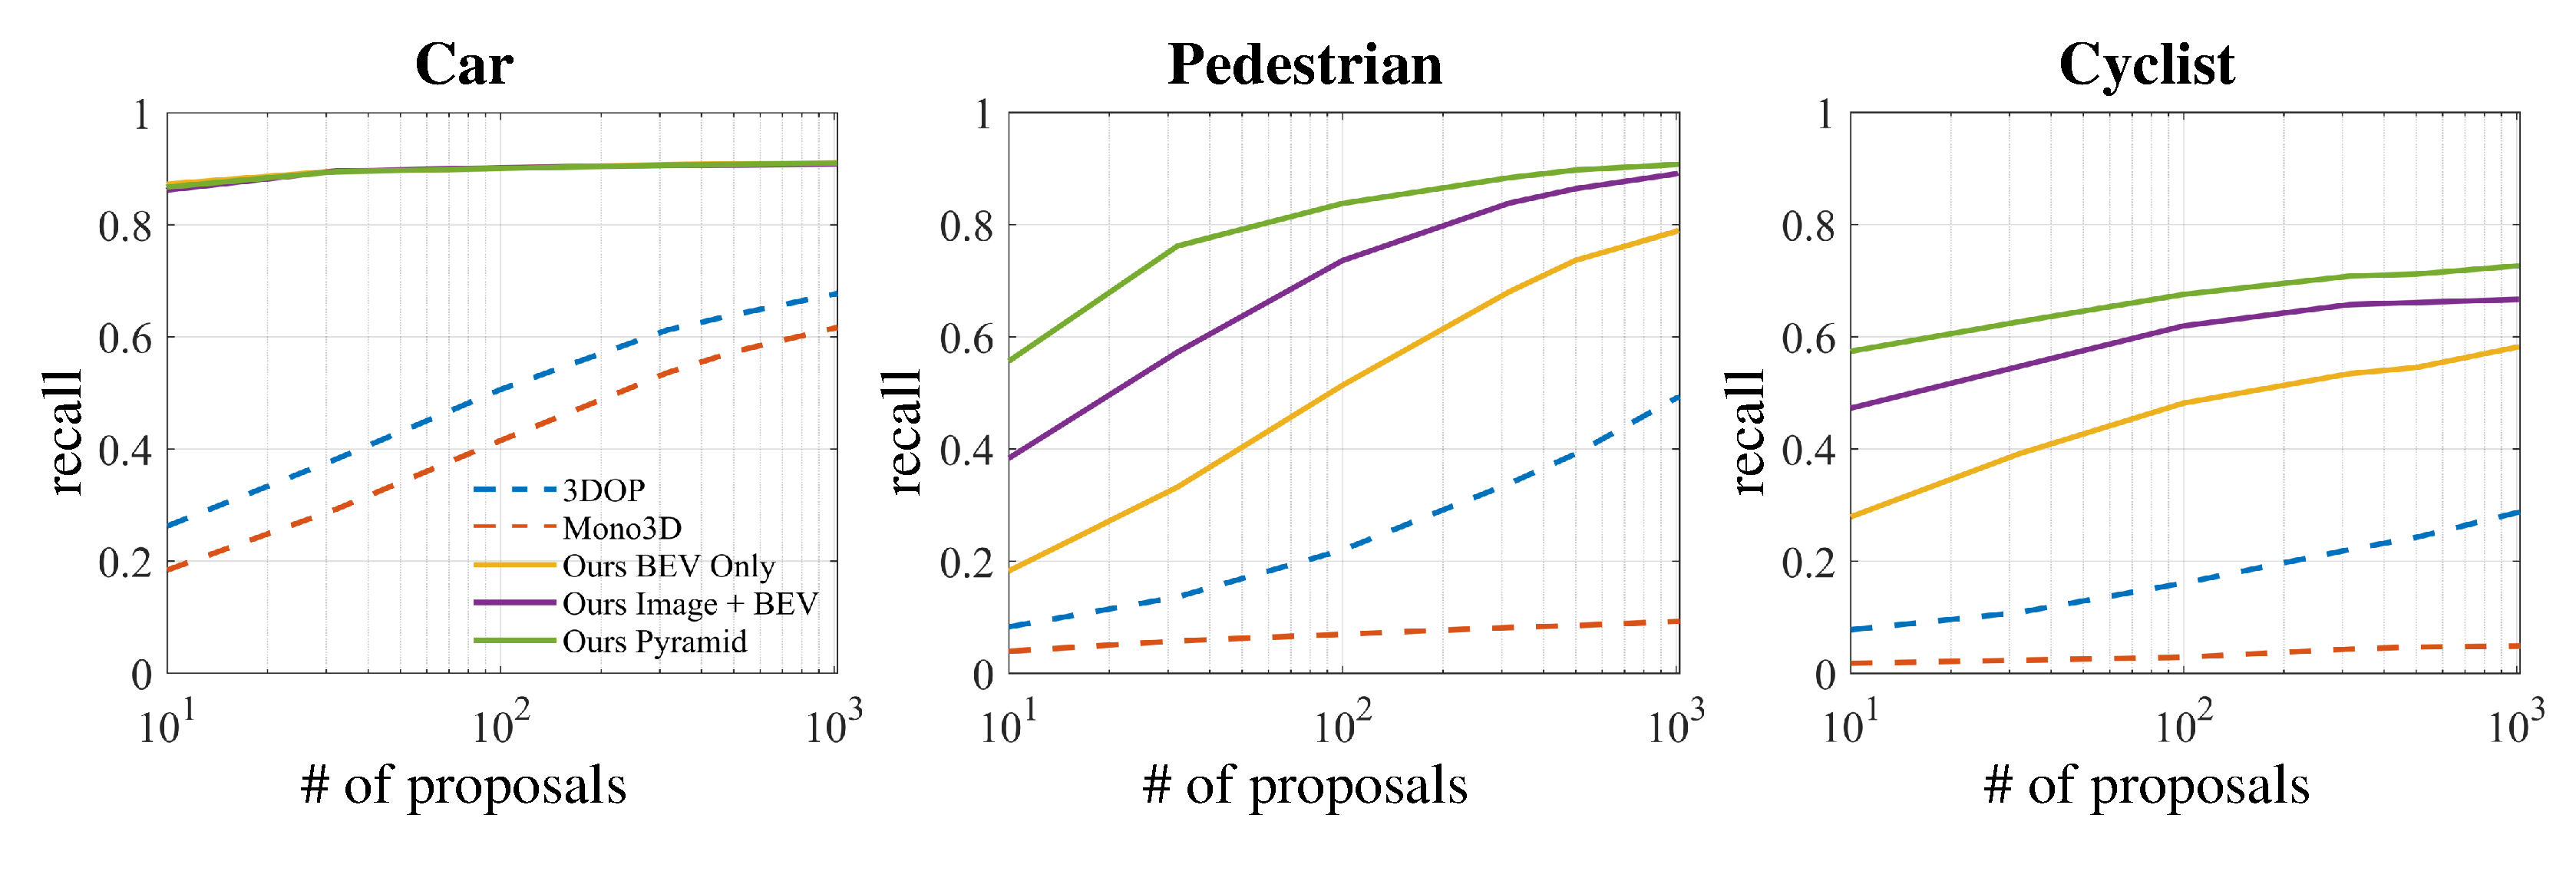
\includegraphics[width=1.08\textwidth]{images/pdfs/RPN_Results.pdf}
			\caption{The recall vs number of proposals at a 3D IoU threshold of 0.5.}
	\end{figure}
\end{frame}

\begin{frame}
	\frametitle{Background: F-PointNet \footnote{Frustum PointNets for 3D Object Detection from RGB-D Data (CVPR) 2018}}
	\begin{figure}
		\begin{center}
			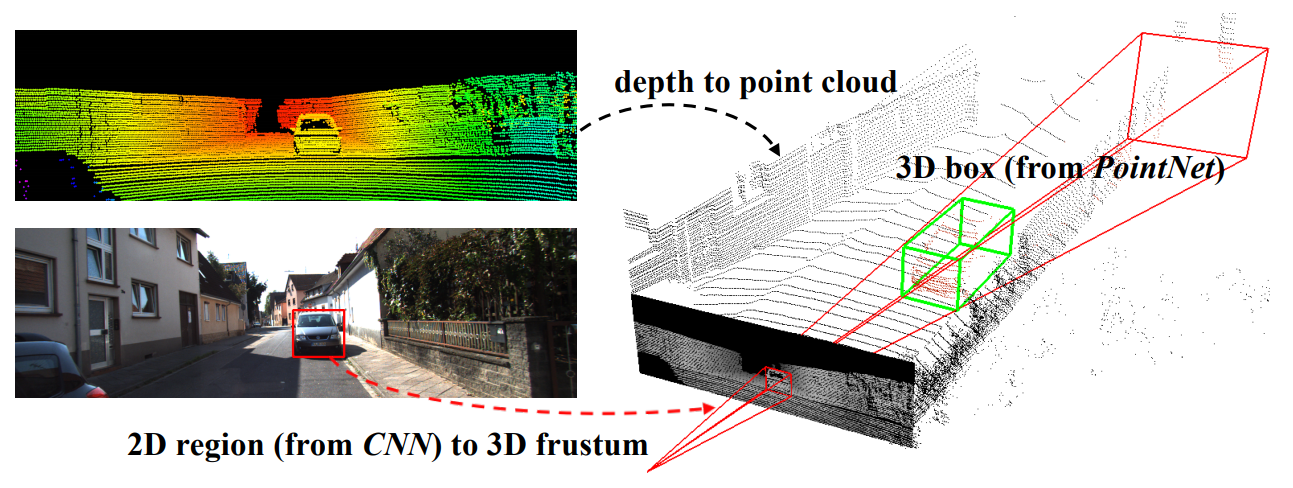
\includegraphics[width=1.0\linewidth]{images/fpoint_net} \\
			%\caption{F-PointNet detection pipeline \cite{}.}
		\end{center}
	\end{figure}
\end{frame}

\begin{frame}
	\frametitle{Background: PointNet}
	\linespread{1.5}
	\begin{itemize}
		\item{Avoid converting pointcloud to other representations}
		\begin{itemize}
		    \item Voxelization
		    \item Projection/Rendering
		    \item Feature extraction
		\end{itemize}
		\item{Pointcloud feature learning}
		\begin{itemize}
	        \item Unordered point set as input
	        \item Invariance under geometric transformations 
		\end{itemize}
	\begin{figure}
		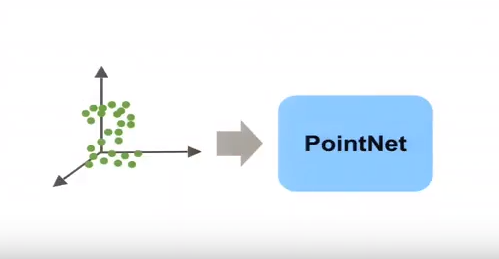
\includegraphics[width=0.5\linewidth]{images/pointnet/pointNet} \\
	\end{figure}
	\end{itemize}
\end{frame}

% HYS: Model needs to be invariant to N! permutations
% Point cloud rotations should not alter results
% How can we construct a family of symmetric functions by NN
\begin{frame}
\frametitle{Permutation Invariance: Symmetric Function}
\linespread{1.5}
	\begin{center}
    \begin{align*}
    	\quad \quad \quad \quad
        f(x_1,x_2,...,x_n) = f(x_{\pi_1},x_{\pi_2},...,x_{\pi_n}), x_i \in \mathbb{R}^D
    \end{align*}
    \end{center}
    \begin{itemize}
        \item \textbf{Examples}:
             \begin{align*}
             	\quad \quad \quad \quad
               f(x_1,x_2,...,x_n) = \max \{x_1,x_2,...,x_n\} \\
               f(x_1,x_2,...,x_n) = x_1 + x_2 + ... +x_n
            \end{align*}
            \item Idea: Construct a family of symmetric functions by neural networks.
    \end{itemize}
\end{frame}

% HYS: Learn and apply an affine transformation to input point coordinates - transformation is predicted by a mini-pointnet (T-Net) end-to-end trained with the rest of the network.
\begin{frame}
	\frametitle{Input Alignment by Transformer Network}
	\linespread{1.5}
    \begin{itemize}
        \item Data dependent transformation for automatic alignment
    \end{itemize}
    \begin{figure}
		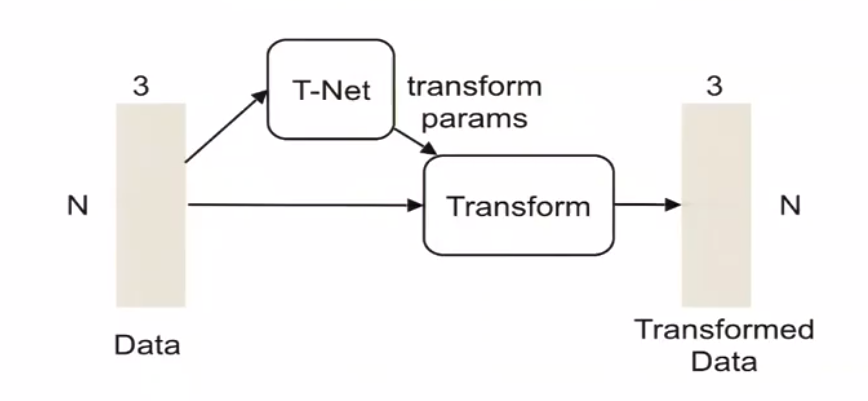
\includegraphics[width=0.8\linewidth]{images/pointnet/t-Net} \\
	\end{figure}
\end{frame}

\begin{frame}
	\frametitle{PointNet Architecture}
	\linespread{1.5}
	\begin{figure}
		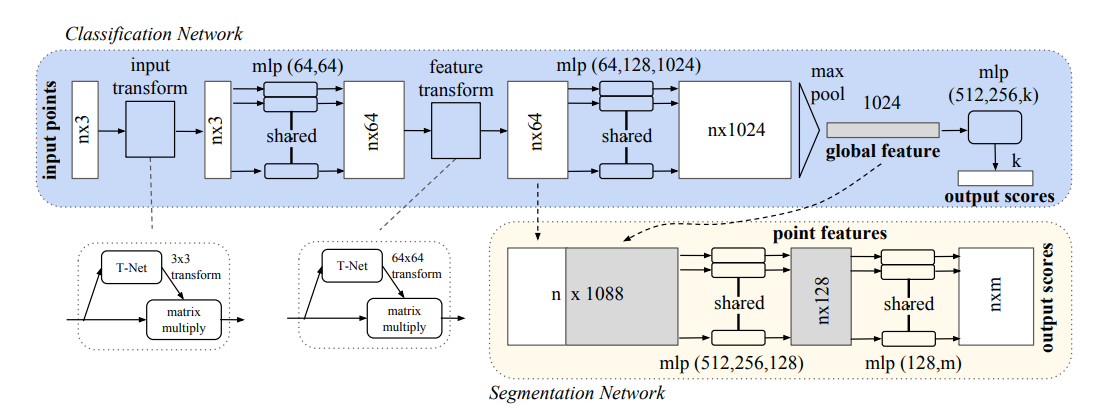
\includegraphics[width=1.0\linewidth]{images/pointnet/pointnet_arch} \\
		\caption{PointNet Classification and Segmentation Network.}
	\end{figure}
\end{frame}

\begin{frame}
	\frametitle{F-PointNet}
	\begin{figure}
		\begin{center}
			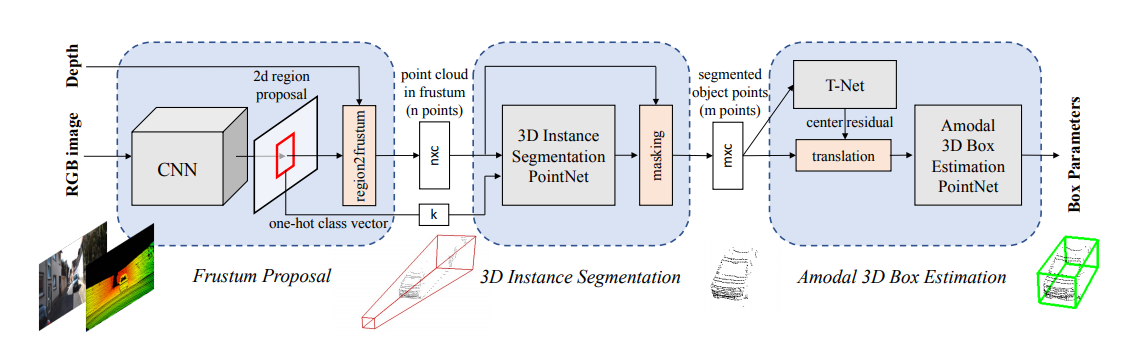
\includegraphics[width=1.0\linewidth]{images/pointnet/fpointNet_arch} \\
			%\caption{F-PointNet detection pipeline \cite{}.}
		\end{center}
	\end{figure}
	\begin{itemize}
	    \item Get a 3D frustum from a 2D image region.
	    \item  Given a point cloud in a frustum, the object instance is segmented.
	    \item T-Net aligns points such that their centroid is close to amodal box center.
	\end{itemize}
\end{frame}

\begin{frame}
	\frametitle{Evaluation Metrics for Object Detection}
	\begin{itemize}
		\item{Average Precision (AP)}
		\begin{itemize}
		    \begin{align*}
				AP = \frac{1}{11} \sum_{r \in{0,0.1,...,1}}^{} p_{interp}(r)\\
				p_{interp}(r) = \max_{\hat{r}:\hat{r} \geq r} p(\hat{r})
			\end{align*}
			\item{where $p(\hat{r})$ is the measured precision at recall $\hat{r}$.}
		\end{itemize}
	\end{itemize}
\end{frame}


\begin{frame}
	\frametitle{AVOD - Results on Car Detection}
\begin{table}
	\begin{tabular}{l | c | c | c | c }
		Method & Moderate & Easy & Hard & Runtime \\
		\hline \hline
		AVOD-FPN & \textbf{71.88} & \textbf{81.94} & \textbf{66.38} & 0.1 \\
		F-PointNet & 70.39 & 81.20 & 62.19  & 0.17 \\ 
		AVOD & 65.78 & 73.59 & 58.38 & \textbf{0.08} \\
		VoxelNet & 65.11 & 77.47 & 57.73 & 0.25 \\
		MV3D & 62.35 & 71.09 & 55.12 & 0.36 \\
	\end{tabular}
	\caption{A comparison of the performance of AVOD with the state of the art 3D object detectors evaluated on KITTI's dataset. Results are generated by KITTI's evaluation server.}
\end{table}
\end{frame}

\begin{frame}
	\frametitle{AVOD - Results on Pedestrian Detection}
	\begin{table}
		\begin{tabular}{l | c | c | c | c }
			Method & Moderate & Easy & Hard & Runtime \\
			\hline \hline
			F-PointNet & \textbf{44.89} & \textbf{51.21} & 40.23 & 0.17 \\
			AVOD-FPN & 42.81 & 50.80 & \textbf{40.88} & 0.1 \\
			VoxelNet & 33.69 & 39.48 & 31.51	 & 0.25 \\ 
			AVOD & 31.51 & 38.28 & 26.98 & \textbf{0.08} \\
		\end{tabular}
		\caption{A comparison of the performance of AVOD with the state of the art 3D object detectors evaluated on KITTI's dataset. Results are generated by KITTI's evaluation server.}
	\end{table}
\end{frame}

\begin{frame}
	\frametitle{AVOD - Results on Cyclist Detection}
	\begin{table}
		\begin{tabular}{l | c | c | c | c }
			Method & Moderate & Easy & Hard & Runtime \\
			\hline \hline
			F-PointNet & \textbf{56.77} & \textbf{71.96} & \textbf{50.39}  & 0.17 \\
			AVOD-FPN & 52.18 & 64.00 & 46.61 & 0.1 \\
			VoxelNet & 48.36 & 61.22 & 44.37 & 0.25 \\ 
			AVOD & 44.90  & 60.11 & 38.80 & \textbf{0.08} \\
		\end{tabular}
		\caption{A comparison of the performance of AVOD with the state of the art 3D object detectors evaluated on KITTI's dataset. Results are generated by KITTI's evaluation server.}
	\end{table}
\end{frame}

\begin{frame}
	\frametitle{AVOD Results on KITTI and Autonomoose}
	\begin{center}
		\movie[width=0.5\textwidth,showcontrols=true]
		{% placeholder = text or image
		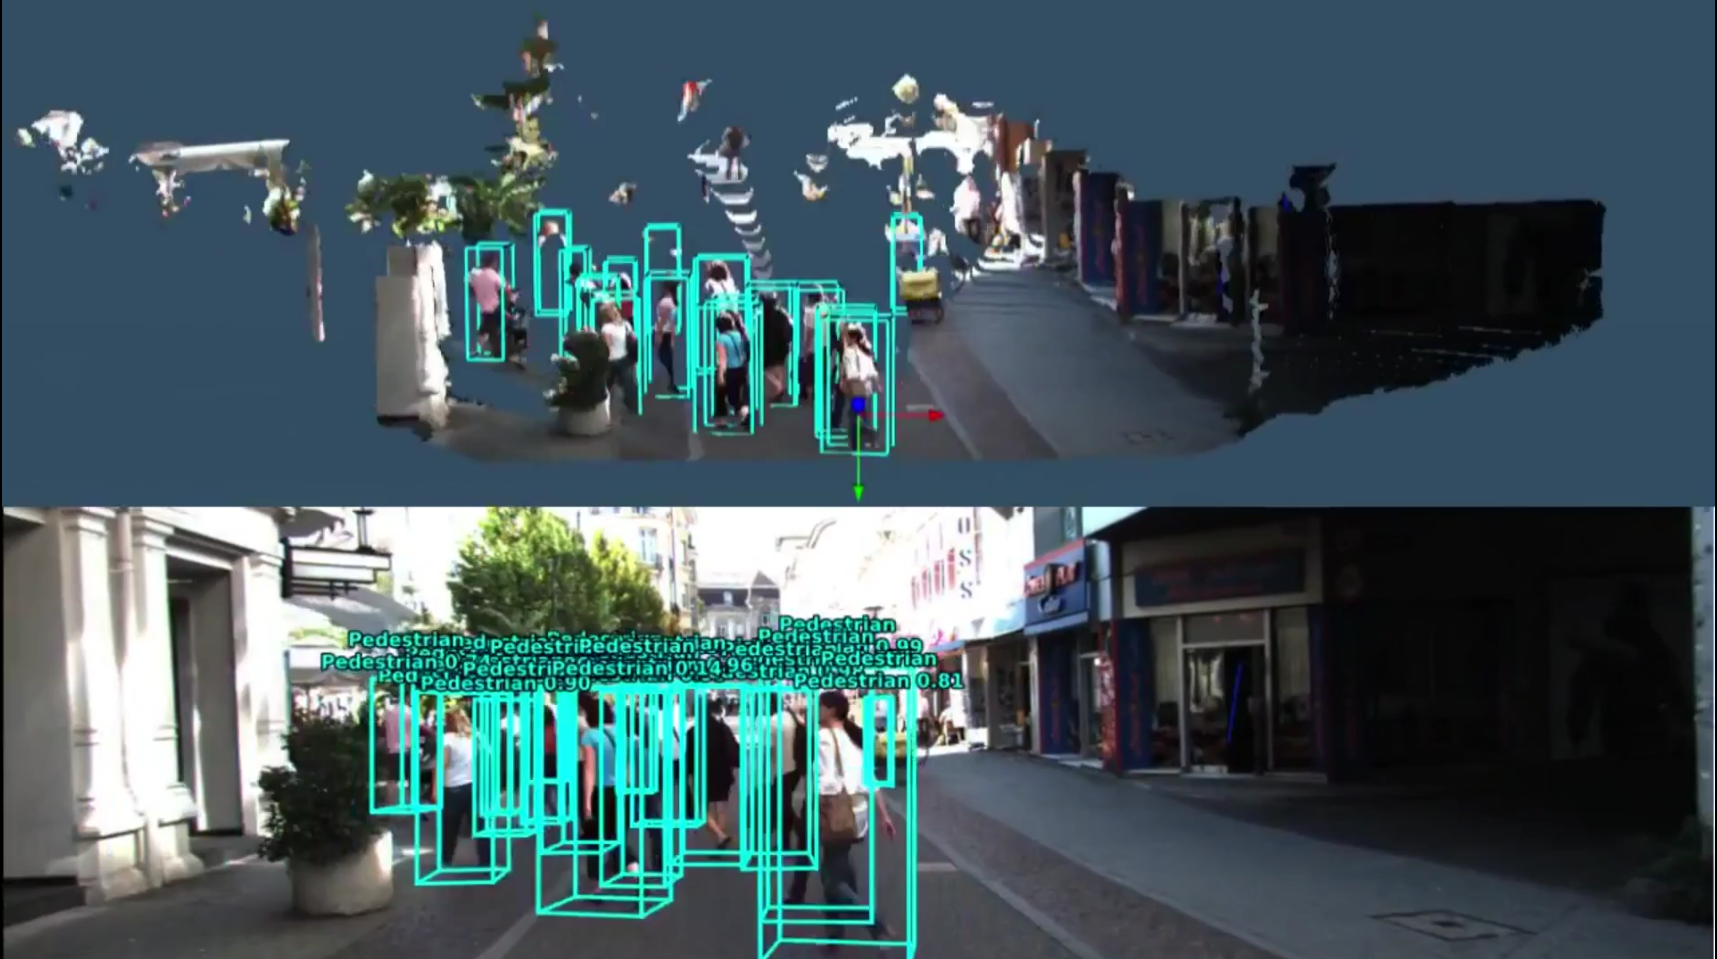
\includegraphics[width=0.7\textwidth]{images/video/video_logo.png}
		}%
		{images/video/AVOD.mp4}
	\end{center}
\end{frame}

\begin{frame}
	\frametitle{Motivation: Single Stage Detector}
	\linespread{1.5}
	\begin{itemize}
		\item{The highest accuracy object detectors to date are based on two-stage detectors.}
		\item{Single stage object detection algorithms are \textit{simple}:}
		\begin{itemize}
			\item{Eliminate proposal generation and feature resampling stage.}
			\item{Encapsulate all computation into a \textbf{single} stage.}
		\end{itemize}
	\end{itemize}
\end{frame}

\section{AVOD-SSD}
\begin{frame}
	\frametitle{AVOD-Single Stage Detector Architecture}
		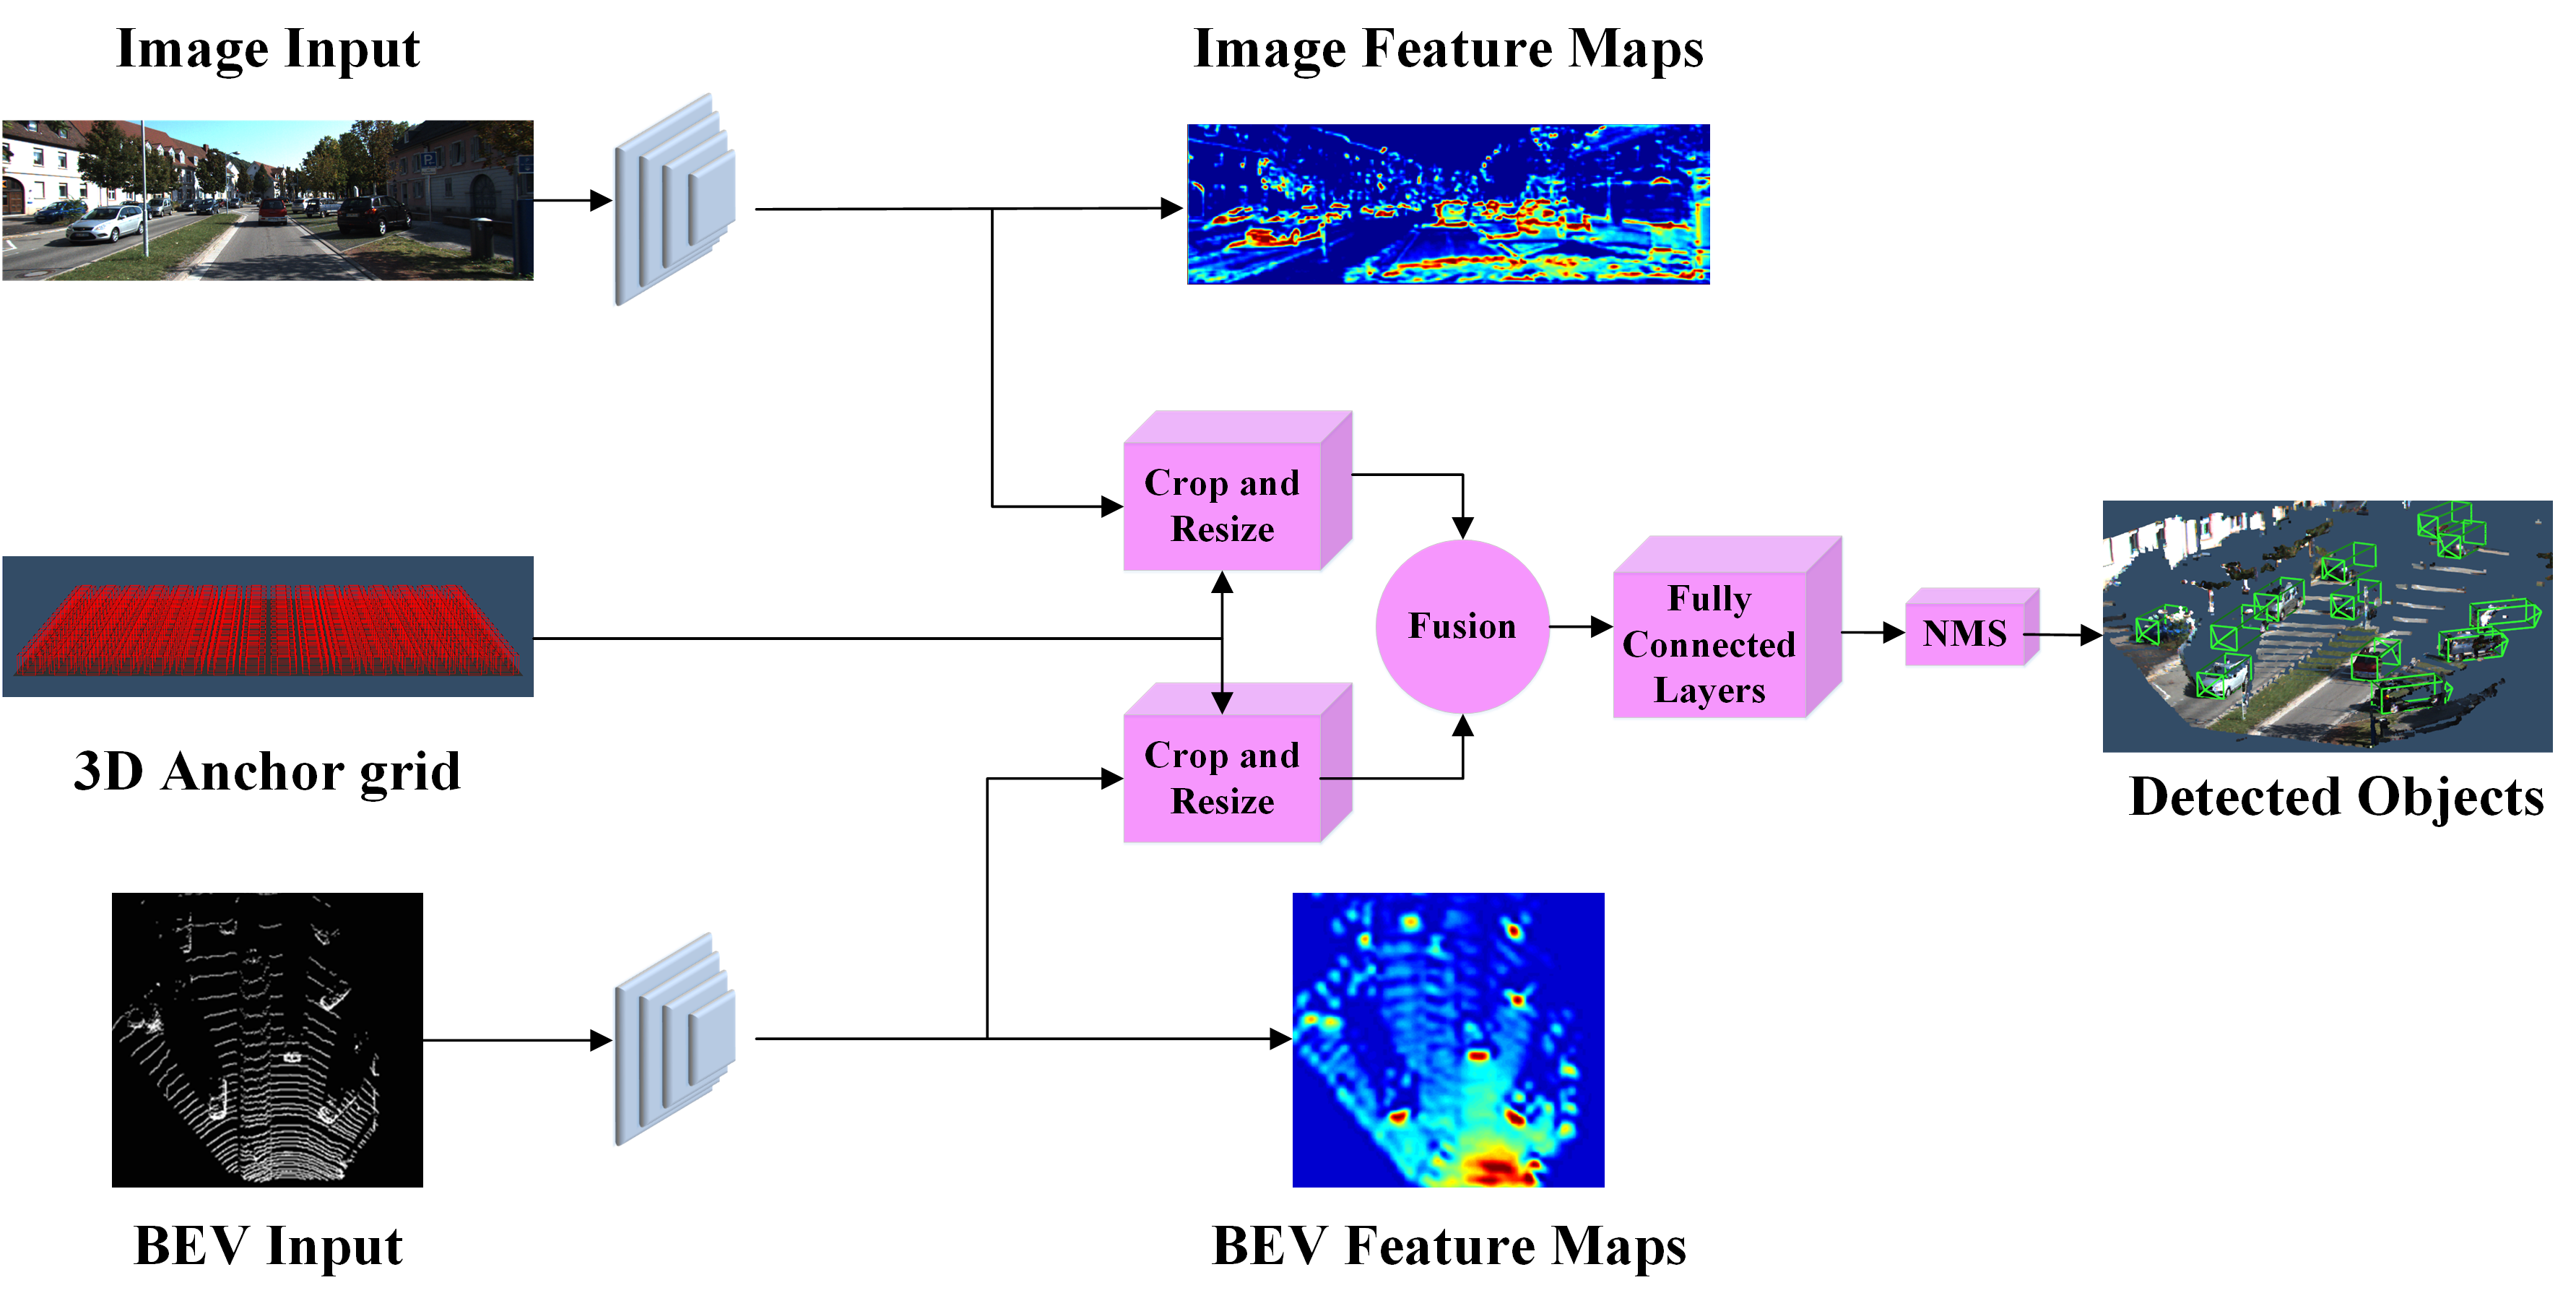
\includegraphics[width=1.0\textwidth]{images/avod_ssd}
\end{frame}


\begin{frame}
	\frametitle{Class Imbalance}
	\linespread{1.5}
	\begin{itemize}
		\item{Evaluate $10 - 100K$ candidate locations but only a few locations contain objects.}
		\item{This imbalance causes two problems: }
		\begin{itemize}
			\item{Training is \textit{inefficient}.}
			\item{Easy negatives are overwhelming.}
		\end{itemize}
		\item{Common solutions:}
		\begin{itemize}
			\item{Hard negative mining.}
			\item{More complex sampling technique.}
		\end{itemize}
	\end{itemize}
\end{frame}


\begin{frame}
	\frametitle{Focal Loss}
	\linespread{1.5}
	\begin{itemize}
		\item{Designed to address class imbalance by down-weighting \textit{easy} examples:}
		\begin{itemize}
			\item{So that their contribution to the total loss is small even if their number is large.}
		\end{itemize}
		\item{Focuses training on \textit{hard} examples.}
	\end{itemize}
\end{frame}

\begin{frame}
	\frametitle{Focal Loss Continued}
	\begin{itemize}
		\item{To introduce the formulation of focal loss, we start with cross entropy (CE) loss for binary classification:}
	\end{itemize}
	\begin{center}
		\begin{align*}
		\quad \quad \quad \quad  \quad \quad
		CE(p,y)= 
		\begin{dcases}
		-log(p),& \text{if } y=1\\
		-log(1-p),              & \text{otherwise}
		\end{dcases}
		\end{align*}
	\end{center}
	\begin{itemize}
		\item{In the above equation $y \in \{\pm 1\}$ specifies the ground-truth class and $p \in [0, 1]$ is the model's estimated probability for the class with label $y=1$.}
	\end{itemize}
\end{frame}


\begin{frame}
	\frametitle{Focal Loss Continued}
	\begin{itemize}
		\item{ For notational convenience, we define $p_t$:}
	\end{itemize}
	\begin{center}
		\begin{align*}
		\quad \quad \quad \quad  \quad \quad \quad \quad
		p_t= 
		\begin{dcases}
		p,& \text{if } y=1\\
		1-p,              & \text{otherwise}
		\end{dcases}
		\end{align*}
	\end{center}
	\begin{itemize}
		\item{Then we can rewrite CE$(p,y) = $ CE$(p_t)$ = $-log(p_t)$.}
	\end{itemize}
\end{frame}

\begin{frame}
	\frametitle{Balanced Cross Entropy}
	\linespread{1.5}
	\begin{itemize}
		\item{Weighting factor $\alpha \in [0,1]$.}
		\item $\alpha$ for class $1$, and $ 1 - \alpha$ for class $-1$.
	\end{itemize}	
	\begin{center}
		\begin{align*}
		\quad \quad \quad \quad  \quad \quad  \quad \quad BCE(p_t) = - \alpha_t log(p_t)
		\end{align*}
	\end{center}
\end{frame}

\begin{frame}
	\frametitle{Focal Loss Definition}
	\linespread{1.5}
	\begin{itemize}
		\item{$\alpha$ balances the importance of \textbf{positive} and \textbf{negative} examples, it does not differentiate between \textbf{easy} and \textbf{hard} examples.}
		\item{Focal loss uses a modulating factor $(1 - p_t)^\gamma$ with the cross entropy loss, with a tunable \textit{focusing} parameter $\gamma \ge 0$.}
	\end{itemize}
	\begin{center}
		\begin{equation*}
		\quad  \quad \quad \quad  \quad \quad \quad \quad FL(p_t) = - \alpha_t (1 - p_t)^\gamma log(p_t)
		\end{equation*}
	\end{center}

\end{frame}

\begin{frame}
	\frametitle{Focal Loss Plot}
	\begin{figure}
		\begin{center}
			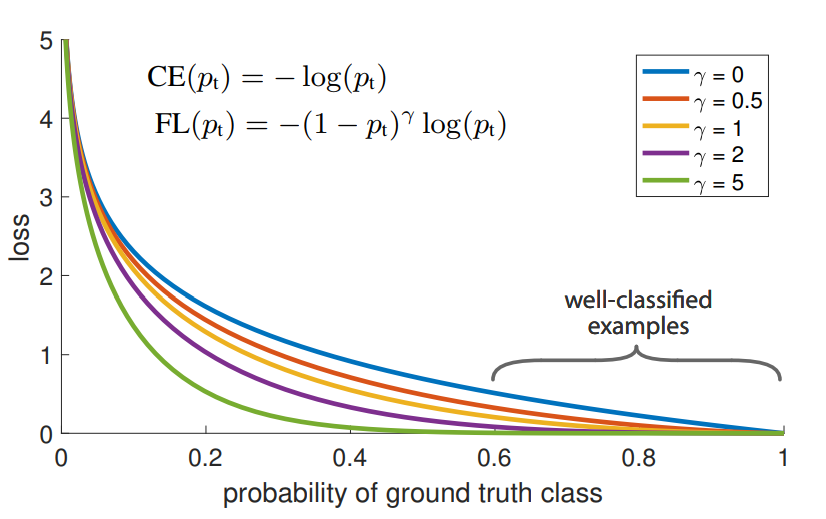
\includegraphics[width=0.8\columnwidth]{images/focal_loss.png}
		\end{center}
		\caption{The focal loss visualized for several values of $\gamma \in [0, 5]$ \cite{focallossRoss}.}
	\end{figure}
\end{frame}


\definecolor{Pink}{cmyk}{0, 0.9808, 0.4429, 0.1412}
\definecolor{Green}{rgb}{0,200,0}

\begin{frame}
\frametitle{AVOD-SSD Experiment Results}
\begin{table}[h]
	\centering
	\resizebox{1.0\textwidth}{!}{
		\begin{tabular}{c c c c}
			\toprule
			&\multicolumn{2}{c}{Car}&\\
			Architecture &  $AP_{3D} (0.7)$ & $AHS_{3D} (0.7)$ & Runtime speed (s)\\
			\midrule
			\midrule
			\rowcolor{Gray}
			AVOD & 74.23 & 73.97 & \textbf{0.08} \\
			
			AVOD-FPN & \textbf{74.81} & \textbf{74.53} & 0.1 \\
			
			AVOD-FPN(High Res BEV) & 73.74 & 73.11 & 0.14 \\
			\rowcolor{Pink}
			AVOD-SSD(FPN) \textbf{without} Focal Loss & 61.52 & 60.32 & 0.09 \\
			\rowcolor{Pink}
			AVOD-SSD(VGG) &  56.11 & 55.89 & 0.2 \\
			\rowcolor{Green}
			AVOD-SSD(FPN) & 73.93 & 73.32 & 0.09 \\
			\rowcolor{Green}
			AVOD-SSD(FPN + High Res BEV) & 74.53 & 74.08 & 0.16 \\
			\bottomrule   
		\end{tabular}
	}
	\caption{Performance analysis of \textbf{AVOD}, \textbf{AVOD-FPN} and \textbf{AVOD-SSD} on the \textit{validation} set and \textit{moderate} difficulty.}
	\label{avodVsSSD}
\end{table}
\end{frame}

\begin{frame}
	\frametitle{AVOD-SSD Experiment Results}
\begin{table}[h]
	\centering
	\resizebox{1.0\textwidth}{!}{
		\begin{tabular}{ccc|ccc|ccc|ccc}
			\multicolumn{3}{c}{} & \multicolumn{3}{c}{$AP_{3D} \ (\%)$} & \multicolumn{3}{c}{$AP_{BEV} (\%)$} & \multicolumn{3}{c}{$AP_{2D} (\%)$}\\
			\midrule
			Method & Runtime (s) & Class & Easy & Moderate & Hard & Easy & Moderate & Hard & Easy & Moderate & Hard \\
			\midrule
			AVOD-FPN & $0.1$ & {\textbf{Car}} & \textbf{81.94} & \textbf{71.88} & \textbf{66.38} & \textbf{88.53} & 83.79 & \textbf{77.90} & \textbf{89.99}  & 87.44  & 80.05 \\
			AVOD & $\textbf{0.08}$ &  & 73.59 & 65.78 & 58.38 & 86.80 & \textbf{85.44} & 77.73 & 89.73  & \textbf{88.08}  & \textbf{80.14} \\
			AVOD-SSD & $0.09$ &  & 73.64 & 63.87 & 56.90 & 86.14 & 77.66 & 75.68 & 88.94  & 85.71  & 78.05 \\
			\bottomrule   
		\end{tabular}
	}
	\caption{Performance analysis of \textbf{AVOD}, \textbf{AVOD-FPN} and \textbf{AVOD-SSD} on the KITTI's evaluation server.}
	\label{fig:ssd_kitti_test_result}
\end{table}
\end{frame}

\begin{frame}
   \frametitle{Recall and Precision of AVOD vs AVOD-SSD}
   \begin{figure}
   \begin{center}
   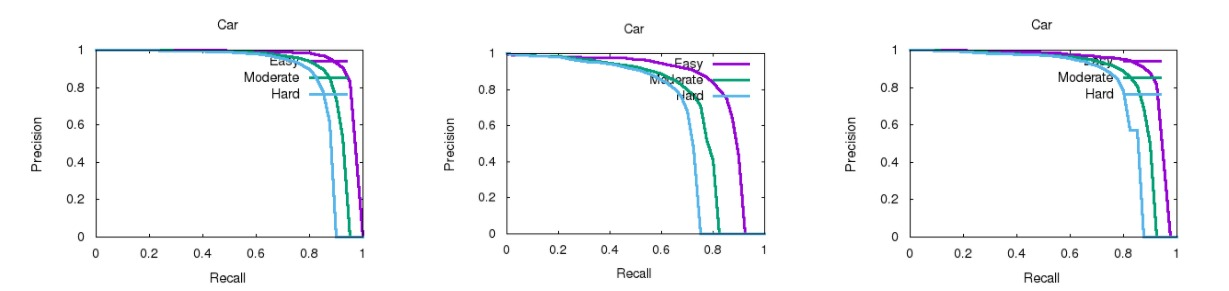
\includegraphics[width=0.9\textwidth]{images/avod_test_plots}\\
   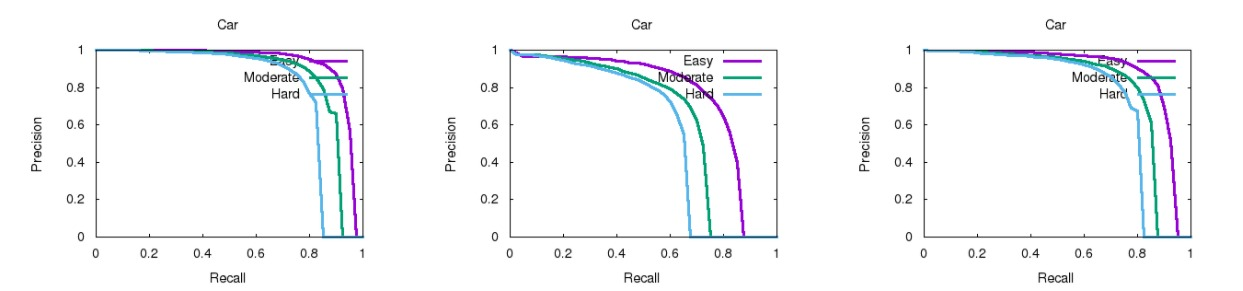
\includegraphics[width=0.9\textwidth]{images/ssd_test_plots}
   \caption{Comparison of Precision-Recall curve of AVOD-FPN(top) vs AVOD-SSD(bottom) for 2D, 3D and BEV detection respectively, on the
      	\textit{test} set.}
   \end{center}
   \end{figure}
\end{frame}

\section{Discussion \& Future Work}
\begin{frame}
	\frametitle{AVOD Limitations}
	\linespread{1.5}
	\begin{itemize}
		\item{2D representation of 3D data}
		\begin{itemize}
			\item{Raw 3D data has much richer information where such information is being discarded.}
%			\item{F-PointNet outperforms AVOD on the task of Pedestrian and Cyclist detection.}
		\end{itemize}
		\item{Accurate estimated ground-plane assumption.}
		\item Objects appear within certain distance above the ground-plane.
	\end{itemize}
\end{frame}

\begin{frame}
	\frametitle{Future Work}
	\linespread{1.5}
	\begin{itemize}
		\item{Speed Optimization}
		\item{Faster 3D Single Stage Detector}
		\item{Processing Temporal Information}
		\begin{itemize}
			\item{Combined pipeline for object detection and tracking where tracking information can also guide object detection and vice versa.}
		\end{itemize}
	\end{itemize}
\end{frame}


\begin{frame}
	\frametitle{References}
	\tiny
	\begin{thebibliography}{9}
		\def\bibfont{\small}
		\bibitem{kitti} 
		Kitti 3D Object Detection Benchmark.
		Access: {\url{http://www.cvlibs.net/datasets/kitti/eval_object.php?obj_benchmark=3d}}.
		
		\bibitem{object_det_cat} 
		Artificial Intelligence GitBook.
		Leonardo Araujo dos Santos.
		Access: {\url{https://leonardoaraujosantos.gitbooks.io/artificial-inteligence/content/object_localization_and_detection.html}}.
		
		\bibitem{faster_rcnn} 
		Faster {R-CNN}: Towards Real-Time Object Detection with Region Proposal Networks.
		Ren, Shaoqing and He, Kaiming and Girshick, Ross and Sun, Jian.
		Access: {\url{https://arxiv.org/abs/1506.01497}}.
		
		\bibitem{vgg_arch} 
		VGG16 Architecture.
		Heuritech.
		Access: {\url{https://blog.heuritech.com/2016/02/29/a-brief-report-of-the-heuritech-deep-learning-meetup-5/}}.
				
		\bibitem{mv3d} 
		Multi-view 3d object detection network for autonomous driving.
		Chen, Xiaozhi and Ma, Huimin and Wan, Ji and Li, Bo and Xia, Tian.
		Access: {\url{https://arxiv.org/abs/1611.07759}}.
		
		\bibitem{frustumpointnet} 
		Frustum PointNets for 3D Object Detection from RGB-D Data.
		Qi, Charles R and Liu, Wei and Wu, Chenxia and Su, Hao and Guibas, Leonidas J.
		Access: {\url{https://arxiv.org/abs/1711.08488}}.
		
		\bibitem{focallossRoss} 
		Focal loss for dense object detection.
		Lin, Tsung-Yi and Goyal, Priya and Girshick, Ross and He, Kaiming and Doll{\'a}r, Piotr.
		Access: {\url{arXiv preprint arXiv:1708.02002}}.
		
		\bibitem{redmon2016you} 
		You only look once: Unified, real-time object detection.
		Redmon, Joseph and Divvala, Santosh and Girshick, Ross and Farhadi, Ali.
		Proceedings of the IEEE conference on computer vision and pattern recognition	
		
	\end{thebibliography}
\end{frame}


\begin{frame}
	\begin{center}
		\huge Thank you! \\ Questions?
	\end{center}
\end{frame}

\end{document}
